\documentclass[11pt,xcolor=table]{beamer}
\usetheme{Boadilla}

\beamertemplatenavigationsymbolsempty

\makeatother
\setbeamertemplate{footline}
{
  \leavevmode%
  \hbox{%
  \begin{beamercolorbox}[wd=.4\paperwidth,ht=2.25ex,dp=1ex,center]{author in head/foot}%
    \usebeamerfont{author in head/foot}\insertshortauthor
  \end{beamercolorbox}%
  \begin{beamercolorbox}[wd=.6\paperwidth,ht=2.25ex,dp=1ex,center]{title in head/foot}%
    \usebeamerfont{title in head/foot}\insertshorttitle\hspace*{3em}
    \insertframenumber{} / \inserttotalframenumber\hspace*{1ex}
  \end{beamercolorbox}}%
  \vskip0pt%
}
\makeatletter
\setbeamertemplate{navigation symbols}{}


\usepackage{tikz}
\usetikzlibrary{arrows,positioning, shapes.symbols,shapes.callouts,patterns,shapes,chains,calc,backgrounds,fadings}
\tikzstyle{state}=[circle,thick,draw=black, align=center, minimum size=2.1cm,
inner sep=0]
\tikzstyle{vertex}=[circle,thick,draw=black]
\tikzstyle{vertex2}=[circle,thick,draw=black,minimum size=0.3cm]
\tikzstyle{vertex3}=[circle,thick,draw=white,minimum size=0.3cm,fill=white]
\tikzstyle{terminal}=[rectangle,thick,draw=black]
\tikzstyle{edge} = [draw,thick]
\tikzstyle{lo} = [edge,dotted]
\tikzstyle{hi} = [edge]
\tikzstyle{trans} = [edge,->]
\tikzstyle{image}=[circle,thick,draw=black]

\newcommand{\hilight}[1]{\colorbox{yellow}{#1}}

\usepackage{graphicx}
\usepackage{caption}
\usepackage{subcaption}

\usepackage{listings} % for listing source code
\lstset{ %
  backgroundcolor=\color{white},   % choose the background color; you must add \usepackage{color} or \usepackage{xcolor}
  basicstyle=\ttfamily,        	    % the size of the fonts that are used for the code
  breakatwhitespace=false,         % sets if automatic breaks should only happen at whitespace
  breaklines=true,                 % sets automatic line breaking
  captionpos=b,                    % sets the caption-position to bottom
  commentstyle=\color{mymauve},    % comment style
  deletekeywords={...},            % if you want to delete keywords from the given language
  escapeinside={\%*}{*)},          % if you want to add LaTeX within your code
  extendedchars=true,              % lets you use non-ASCII characters; for 8-bits encodings only, does not work with UTF-8
  frame=single,                    % adds a frame around the code
  keepspaces=true,                 % keeps spaces in text, useful for keeping indentation of code (possibly needs columns=flexible)
  keywordstyle=\color{blue},       % keyword style
  language=C++,                    % the language of the code
  morekeywords={*,...},            % if you want to add more keywords to the set
  numbers=left,                    % where to put the line-numbers; possible values are (none, left, right)
  numbersep=5pt,                   % how far the line-numbers are from the code
  numberstyle=\tiny\color{mygray}, % the style that is used for the line-numbers
  rulecolor=\color{black},         % if not set, the frame-color may be changed on line-breaks within not-black text (e.g. comments (green here))
  showspaces=false,                % show spaces everywhere adding particular underscores; it overrides 'showstringspaces'
  showstringspaces=false,          % underline spaces within strings only
  showtabs=false,                  % show tabs within strings adding particular underscores
  stepnumber=2,                    % the step between two line-numbers. If it's 1, each line will be numbered
  stringstyle=\color{mymauve},     % string literal style
  tabsize=2,                       % sets default tabsize to 2 spaces
  title=\lstname                   % show the filename of files included with \lstinputlisting; also try caption instead of title
}

% \usepackage[table,usenames,dvipsnames]{xcolor} % for coloured cells in tables

\definecolor{blue3}{HTML}{86B7FC} % med blue
\definecolor{blue1}{HTML}{B5F1FF} % light blue
\definecolor{blue2}{HTML}{E0F9FF} % very light blue
\definecolor{darkgreen2}{HTML}{164816} % dark green

\definecolor{darkgreen}{HTML}{000000} % dark green


\newcommand{\gscaling}{0.7}

\newcommand{\gone}{
    \begin{tabular}{>{\centering\bfseries}m{1in} >{\centering}m{0in}}	
      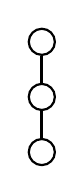
\begin{tikzpicture}[scale=\gscaling,auto,swap]

	% define the round nodes
	\foreach \pos/\name/\label in {
	  {(0,1)//1a},
	  {(0,0)//2a},
	  {(0,-1)//3a}}
	  \node[vertex2] (\label) at \pos {$\name$} ;

	%neighbouring graph
	      
	\path[hi, line width=1.0]  (1a)  -- (2a);
	\path[hi, line width=1.0]  (2a)  -- (3a);

	
      \end{tikzpicture} & \Large{$G_{1}$}
    \end{tabular}
}

\newcommand{\gonecca}[1]{
    \begin{tabular}{>{\centering\bfseries}m{0.4in} >{\centering}m{0in}}	
      \begin{tikzpicture}[scale=\gscaling,auto,swap]

	% define the round nodes
	\foreach \pos/\name/\label in {
	  {(0,1)//1a},
	  {(0,0)//2a},
	  {(0,-1)//3a}}
	  \node[vertex2,draw=#1,fill=#1] (\label) at \pos {$\name$} ;

	%neighbouring graph
	      
	\path[hi, line width=1.0,draw=#1]  (1a)  -- (2a);
	\path[hi, line width=1.0,draw=#1]  (2a)  -- (3a);

	
      \end{tikzpicture} \cellcolor{black} & \cellcolor{black}\textcolor{white}{\Large{$G_{1}$}}
    \end{tabular}
}

\newcommand{\gtwo}{
    \begin{tabular}{>{\centering\bfseries}m{1in} >{\centering}m{0in}}	
      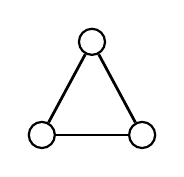
\begin{tikzpicture}[scale=\gscaling * 1.3,auto,swap]

	% define the round nodes
	\foreach \pos/\name/\label in {
	  {(0,1.3)//1a},
	  {(-0.7,0)//2a},
	  {(0.7,0)//3a}}
	  \node[vertex2] (\label) at \pos {$\name$} ;

	%neighbouring graph
	      
	\path[hi, line width=1.0]  (1a)  -- (2a);
	\path[hi, line width=1.0]  (2a)  -- (3a);
	\path[hi, line width=1.0]  (3a)  -- (1a);

	
      \end{tikzpicture} & \Large{$G_{2}$}
    \end{tabular}
}

\newcommand{\gtwopic}{	
      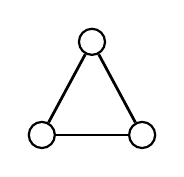
\begin{tikzpicture}[scale=\gscaling * 1.3,auto,swap]

	% define the round nodes
	\foreach \pos/\name/\label in {
	  {(0,1.3)//1a},
	  {(-0.7,0)//2a},
	  {(0.7,0)//3a}}
	  \node[vertex2] (\label) at \pos {$\name$} ;

	%neighbouring graph
	      
	\path[hi, line width=1.0]  (1a)  -- (2a);
	\path[hi, line width=1.0]  (2a)  -- (3a);
	\path[hi, line width=1.0]  (3a)  -- (1a);

	
      \end{tikzpicture}
}


\newcommand{\gtwocca}[1]{
    \begin{tabular}{>{\centering\bfseries}m{0.7in} >{\centering}m{0in}}	
      \begin{tikzpicture}[scale=\gscaling * 1.3,auto,swap]

	% define the round nodes
	\foreach \pos/\name/\label in {
	  {(0,1.3)//1a},
	  {(-0.7,0)//2a},
	  {(0.7,0)//3a}}
	  \node[vertex3,draw=#1,fill=#1] (\label) at \pos {$\name$} ;

	%neighbouring graph
	      
	\path[hi, line width=1.0,draw=#1]  (1a)  -- (2a);
	\path[hi, line width=1.0,draw=#1]  (2a)  -- (3a);
	\path[hi, line width=1.0,draw=#1]  (3a)  -- (1a);

	
      \end{tikzpicture} \cellcolor{black} & \cellcolor{black}\textcolor{white}{\Large{$G_{2}$}}
    \end{tabular}
}

\newcommand{\gfive}{
    \begin{tabular}{>{\centering\bfseries}m{1in} >{\centering}m{0in}}	
      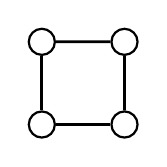
\begin{tikzpicture}[scale=\gscaling * 1.5,auto,swap]

	% define the round nodes
	\foreach \pos/\name/\label in {
	  {(0,0)//1a},
	  {(0,1)//2a},
	  {(1,1)//3a},
	  {(1,0)//4a}}
	  \node[vertex2] (\label) at \pos {$\name$} ;

	%neighbouring graph
	      
	\path[hi, line width=1.0]  (1a)  -- (2a);
	\path[hi, line width=1.0]  (2a)  -- (3a);
	\path[hi, line width=1.0]  (3a)  -- (4a);
	\path[hi, line width=1.0]  (1a)  -- (4a);


	
      \end{tikzpicture} & \Large{$G_{5}$}
    \end{tabular}
}

\newcommand{\gsix}{
    \begin{tabular}{>{\centering\bfseries}m{1in} >{\centering}m{0in}}	
      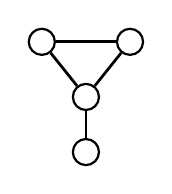
\begin{tikzpicture}[scale=\gscaling,auto,swap]

	% define the round nodes
	\foreach \pos/\name/\label in {
	  {(0,0)//1a},
	  {(-0.8,1)//2a},
	  {(0.8,1)//3a},
	  {(0,-1)//4a}}
	  \node[vertex2] (\label) at \pos {$\name$} ;

	%neighbouring graph
	      
	\path[hi, line width=1.0]  (1a)  -- (2a);
	\path[hi, line width=1.0]  (2a)  -- (3a);
	\path[hi, line width=1.0]  (1a)  -- (3a);
	\path[hi, line width=1.0]  (1a)  -- (4a);


	
      \end{tikzpicture} & \Large{$G_{6}$}
    \end{tabular}
}


\newcommand{\gsixcca}[1]{
    \begin{tabular}{>{\centering\bfseries}m{0.7in} >{\centering}m{0in}}	
      \begin{tikzpicture}[scale=\gscaling,auto,swap]

	% define the round nodes
	\foreach \pos/\name/\label in {
	  {(0,0)//1a},
	  {(-0.8,1)//2a},
	  {(0.8,1)//3a},
	  {(0,-1)//4a}}
	  \node[vertex2,draw=#1,fill=#1] (\label) at \pos {$\name$} ;

	%neighbouring graph
	      
	\path[hi, line width=1.0,draw=#1]  (1a)  -- (2a);
	\path[hi, line width=1.0,draw=#1]  (2a)  -- (3a);
	\path[hi, line width=1.0,draw=#1]  (1a)  -- (3a);
	\path[hi, line width=1.0,draw=#1]  (1a)  -- (4a);


	
      \end{tikzpicture} \cellcolor{black} & \cellcolor{black}\textcolor{white}{\Large{$G_{6}$}}
    \end{tabular}
}

\newcommand{\gseven}{
    \begin{tabular}{>{\centering\bfseries}m{1in} >{\centering}m{0in}}	
      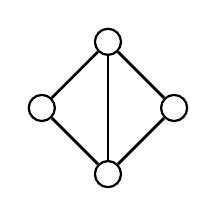
\begin{tikzpicture}[scale=\gscaling * 1.2,auto,swap]

	% define the round nodes
	\foreach \pos/\name/\label in {
	  {(-1.0,0)//1a},
	  {(1,0)//2a},
	  {(0,1)//3a},
	  {(0,-1)//4a}}
	  \node[vertex2] (\label) at \pos {$\name$} ;

	%neighbouring graph
	      
	\path[hi, line width=1.0]  (1a)  -- (3a);
	\path[hi, line width=1.0]  (1a)  -- (4a);
	\path[hi, line width=1.0]  (2a)  -- (3a);
	\path[hi, line width=1.0]  (2a)  -- (4a);
	\path[hi, line width=1.0]  (3a)  -- (4a);

	
      \end{tikzpicture} & \Large{$G_{7}$}
    \end{tabular}
}


\newcommand{\gsevenpic}{
      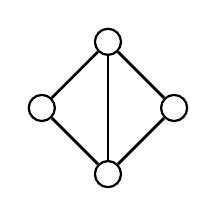
\begin{tikzpicture}[scale=\gscaling * 1.2,auto,swap]

	% define the round nodes
	\foreach \pos/\name/\label in {
	  {(-1.0,0)//1a},
	  {(1,0)//2a},
	  {(0,1)//3a},
	  {(0,-1)//4a}}
	  \node[vertex2] (\label) at \pos {$\name$} ;

	%neighbouring graph
	      
	\path[hi, line width=1.0]  (1a)  -- (3a);
	\path[hi, line width=1.0]  (1a)  -- (4a);
	\path[hi, line width=1.0]  (2a)  -- (3a);
	\path[hi, line width=1.0]  (2a)  -- (4a);
	\path[hi, line width=1.0]  (3a)  -- (4a);

	
      \end{tikzpicture}
}


\newcommand{\geight}{
    \begin{tabular}{>{\centering\bfseries}m{1in} >{\centering}m{0in}}	
      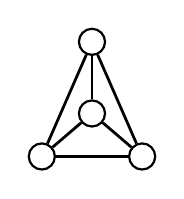
\begin{tikzpicture}[scale=\gscaling * 1.3,auto,swap]

	% define the round nodes
	\foreach \pos/\name/\label in {
	  {(0,0)//1a},
	  {(-0.7,-0.6)//2a},
	  {(0.7,-0.6)//3a},
	  {(0,1)//4a}}
	  \node[vertex2] (\label) at \pos {$\name$} ;

	%neighbouring graph
	      
	\path[hi, line width=1.0]  (1a)  -- (2a);
	\path[hi, line width=1.0]  (1a)  -- (3a);
	\path[hi, line width=1.0]  (1a)  -- (4a);
	\path[hi, line width=1.0]  (2a)  -- (3a);
	\path[hi, line width=1.0]  (2a)  -- (4a);
	\path[hi, line width=1.0]  (3a)  -- (4a);

	
      \end{tikzpicture} & \Large{$G_{8}$}
    \end{tabular}
}


\newcommand{\geightpic}{
      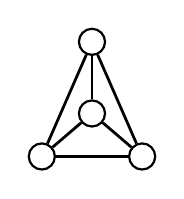
\begin{tikzpicture}[scale=\gscaling * 1.3,auto,swap]

	% define the round nodes
	\foreach \pos/\name/\label in {
	  {(0,0)//1a},
	  {(-0.7,-0.6)//2a},
	  {(0.7,-0.6)//3a},
	  {(0,1)//4a}}
	  \node[vertex2] (\label) at \pos {$\name$} ;

	%neighbouring graph
	      
	\path[hi, line width=1.0]  (1a)  -- (2a);
	\path[hi, line width=1.0]  (1a)  -- (3a);
	\path[hi, line width=1.0]  (1a)  -- (4a);
	\path[hi, line width=1.0]  (2a)  -- (3a);
	\path[hi, line width=1.0]  (2a)  -- (4a);
	\path[hi, line width=1.0]  (3a)  -- (4a);

	
      \end{tikzpicture}
}


\newcommand{\geightcca}[1]{
    \begin{tabular}{>{\centering\bfseries}m{0.7in} >{\centering}m{0in}}	
      \begin{tikzpicture}[scale=\gscaling * 1.3,auto,swap]

	% define the round nodes
	\foreach \pos/\name/\label in {
	  {(0,0)//1a},
	  {(-0.7,-0.6)//2a},
	  {(0.7,-0.6)//3a},
	  {(0,1)//4a}}
	  \node[vertex3,draw=#1,fill=#1] (\label) at \pos {$\name$} ;

	%neighbouring graph
	      
	\path[hi, line width=1.0,draw=#1]  (1a)  -- (2a);
	\path[hi, line width=1.0,draw=#1]  (1a)  -- (3a);
	\path[hi, line width=1.0,draw=#1]  (1a)  -- (4a);
	\path[hi, line width=1.0,draw=#1]  (2a)  -- (3a);
	\path[hi, line width=1.0,draw=#1]  (2a)  -- (4a);
	\path[hi, line width=1.0,draw=#1]  (3a)  -- (4a);

	
      \end{tikzpicture} \cellcolor{black} & \cellcolor{black}\textcolor{white}{\Large{$G_{8}$}}
    \end{tabular}
}

\newcommand{\gnine}{
    \begin{tabular}{>{\centering\bfseries}m{1in} >{\centering}m{0in}}	
      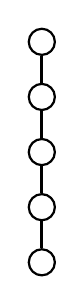
\begin{tikzpicture}[scale=\gscaling,auto,swap]

	% define the round nodes
	\foreach \pos/\name/\label in {
	  {(0,2)//1a},
	  {(0,1)//2a},
	  {(0,0)//3a},
	  {(0,-1)//4a},
	  {(0,-2)//5a}}
	  \node[vertex2] (\label) at \pos {$\name$} ;

	%neighbouring graph
	      
	\path[hi, line width=1.0]  (1a)  -- (2a);
	\path[hi, line width=1.0]  (2a)  -- (3a);
	\path[hi, line width=1.0]  (3a)  -- (4a);
	\path[hi, line width=1.0]  (4a)  -- (5a);


	
      \end{tikzpicture} & \Large{$G_{9}$}
    \end{tabular}
}

\newcommand{\gninepic}{
      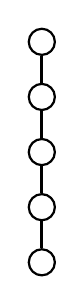
\begin{tikzpicture}[scale=\gscaling,auto,swap]

	% define the round nodes
	\foreach \pos/\name/\label in {
	  {(0,2)//1a},
	  {(0,1)//2a},
	  {(0,0)//3a},
	  {(0,-1)//4a},
	  {(0,-2)//5a}}
	  \node[vertex2] (\label) at \pos {$\name$} ;

	%neighbouring graph
	      
	\path[hi, line width=1.0]  (1a)  -- (2a);
	\path[hi, line width=1.0]  (2a)  -- (3a);
	\path[hi, line width=1.0]  (3a)  -- (4a);
	\path[hi, line width=1.0]  (4a)  -- (5a);


	
      \end{tikzpicture}
}

\newcommand{\gninecca}[1]{
    \begin{tabular}{>{\centering\bfseries}m{0.7in} >{\centering}m{0in}}	
      \begin{tikzpicture}[scale=\gscaling,auto,swap]

	% define the round nodes
	\foreach \pos/\name/\label in {
	  {(0,2)//1a},
	  {(0,1)//2a},
	  {(0,0)//3a},
	  {(0,-1)//4a},
	  {(0,-2)//5a}}
	  \node[vertex3,draw=#1,fill=#1] (\label) at \pos {$\name$} ;

	%neighbouring graph
	      
	\path[hi, line width=1.0,draw=#1]  (1a)  -- (2a);
	\path[hi, line width=1.0,draw=#1]  (2a)  -- (3a);
	\path[hi, line width=1.0,draw=#1]  (3a)  -- (4a);
	\path[hi, line width=1.0,draw=#1]  (4a)  -- (5a);


	
      \end{tikzpicture} \cellcolor{black} & \cellcolor{black}\textcolor{white}{\Large{$G_{9}$}}
    \end{tabular}
}


\newcommand{\gten}{
    \begin{tabular}{>{\centering\bfseries}m{1in} >{\centering}m{0in}}	
      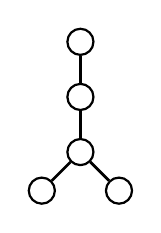
\begin{tikzpicture}[scale=\gscaling,auto,swap]

	% define the round nodes
	\foreach \pos/\name/\label in {
	  {(0,2)//1a},
	  {(0,1)//2a},
	  {(0,0)//3a},
	  {(-0.7,-0.7)//4a},
	  {(0.7,-0.7)//5a}}
	  \node[vertex2] (\label) at \pos {$\name$} ;

	%neighbouring graph
	      
	\path[hi, line width=1.0]  (1a)  -- (2a);
	\path[hi, line width=1.0]  (2a)  -- (3a);
	\path[hi, line width=1.0]  (3a)  -- (4a);
	\path[hi, line width=1.0]  (3a)  -- (5a);


	
      \end{tikzpicture} & \Large{$G_{10}$}
    \end{tabular}
}

\newcommand{\gtenpic}{
      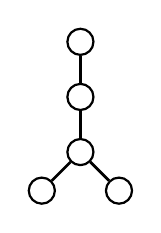
\begin{tikzpicture}[scale=\gscaling,auto,swap]

	% define the round nodes
	\foreach \pos/\name/\label in {
	  {(0,2)//1a},
	  {(0,1)//2a},
	  {(0,0)//3a},
	  {(-0.7,-0.7)//4a},
	  {(0.7,-0.7)//5a}}
	  \node[vertex2] (\label) at \pos {$\name$} ;

	%neighbouring graph
	      
	\path[hi, line width=1.0]  (1a)  -- (2a);
	\path[hi, line width=1.0]  (2a)  -- (3a);
	\path[hi, line width=1.0]  (3a)  -- (4a);
	\path[hi, line width=1.0]  (3a)  -- (5a);


	
      \end{tikzpicture}
}


\newcommand{\gtencca}[1]{
    \begin{tabular}{>{\centering\bfseries}m{0.7in} >{\centering}m{0in}}	
      \begin{tikzpicture}[scale=\gscaling,auto,swap]

	% define the round nodes
	\foreach \pos/\name/\label in {
	  {(0,2)//1a},
	  {(0,1)//2a},
	  {(0,0)//3a},
	  {(-0.7,-0.7)//4a},
	  {(0.7,-0.7)//5a}}
	  \node[vertex3,draw=#1,fill=#1] (\label) at \pos {$\name$} ;

	%neighbouring graph
	      
	\path[hi, line width=1.0,draw=#1]  (1a)  -- (2a);
	\path[hi, line width=1.0,draw=#1]  (2a)  -- (3a);
	\path[hi, line width=1.0,draw=#1]  (3a)  -- (4a);
	\path[hi, line width=1.0,draw=#1]  (3a)  -- (5a);


	
      \end{tikzpicture} \cellcolor{black} & \cellcolor{black}\textcolor{white}{\Large{$G_{10}$}}
    \end{tabular}
}

\newcommand{\geleven}{
    \begin{tabular}{>{\centering\bfseries}m{1in} >{\centering}m{0in}}	
      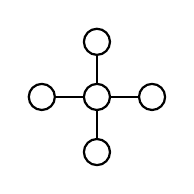
\begin{tikzpicture}[scale=\gscaling,auto,swap]

	% define the round nodes
	\foreach \pos/\name/\label in {
	  {(0,0)//1a},
	  {(0,1)//2a},
	  {(-1,0)//3a},
	  {(0,-1)//4a},
	  {(1,0)//5a}}
	  \node[vertex2] (\label) at \pos {$\name$} ;

	%neighbouring graph
	      
	\path[hi, line width=1.0]  (1a)  -- (2a);
	\path[hi, line width=1.0]  (1a)  -- (3a);
	\path[hi, line width=1.0]  (1a)  -- (4a);
	\path[hi, line width=1.0]  (1a)  -- (5a);


	
      \end{tikzpicture} & \Large{$G_{11}$}
    \end{tabular}
}

\newcommand{\gelevenpic}{
      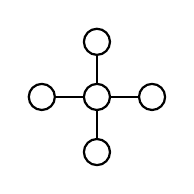
\begin{tikzpicture}[scale=\gscaling,auto,swap]

	% define the round nodes
	\foreach \pos/\name/\label in {
	  {(0,0)//1a},
	  {(0,1)//2a},
	  {(-1,0)//3a},
	  {(0,-1)//4a},
	  {(1,0)//5a}}
	  \node[vertex2] (\label) at \pos {$\name$} ;

	%neighbouring graph
	      
	\path[hi, line width=1.0]  (1a)  -- (2a);
	\path[hi, line width=1.0]  (1a)  -- (3a);
	\path[hi, line width=1.0]  (1a)  -- (4a);
	\path[hi, line width=1.0]  (1a)  -- (5a);


	
      \end{tikzpicture} 

}



\newcommand{\gelevencca}[1]{
    \begin{tabular}{>{\centering\bfseries}m{0.7in} >{\centering}m{0in}}	
      \begin{tikzpicture}[scale=\gscaling,auto,swap]

	% define the round nodes
	\foreach \pos/\name/\label in {
	  {(0,0)//1a},
	  {(0,1)//2a},
	  {(-1,0)//3a},
	  {(0,-1)//4a},
	  {(1,0)//5a}}
	  \node[vertex2,draw=#1,fill=#1] (\label) at \pos {$\name$} ;

	%neighbouring graph
	      
	\path[hi, line width=1.0,draw=#1]  (1a)  -- (2a);
	\path[hi, line width=1.0,draw=#1]  (1a)  -- (3a);
	\path[hi, line width=1.0,draw=#1]  (1a)  -- (4a);
	\path[hi, line width=1.0,draw=#1]  (1a)  -- (5a);


	
      \end{tikzpicture} \cellcolor{black}& \cellcolor{black}\textcolor{white}{\Large{$G_{11}$}}
    \end{tabular}
}


\newcommand{\gtwelve}{
    \begin{tabular}{>{\centering\bfseries}m{1in} >{\centering}m{0in}}	
      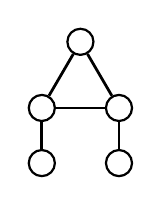
\begin{tikzpicture}[scale=\gscaling,auto,swap]

	% define the round nodes
	\foreach \pos/\name/\label in {
	  {(-0.7,0)//1a},
	  {(0.7,0)//2a},
	  {(0,1.2)//3a},
	  {(-0.7,-1)//4a},
	  {(0.7,-1)//5a}}
	  \node[vertex2] (\label) at \pos {$\name$} ;

	%neighbouring graph
	      
	\path[hi, line width=1.0]  (1a)  -- (2a);
	\path[hi, line width=1.0]  (2a)  -- (3a);
	\path[hi, line width=1.0]  (1a)  -- (3a);
	\path[hi, line width=1.0]  (1a)  -- (4a);
	\path[hi, line width=1.0]  (2a)  -- (5a);

	
      \end{tikzpicture} & \Large{$G_{12}$}
    \end{tabular}
}

\newcommand{\gtwelvepic}{
      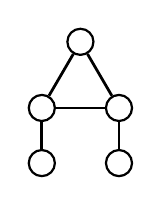
\begin{tikzpicture}[scale=\gscaling,auto,swap]

	% define the round nodes
	\foreach \pos/\name/\label in {
	  {(-0.7,0)//1a},
	  {(0.7,0)//2a},
	  {(0,1.2)//3a},
	  {(-0.7,-1)//4a},
	  {(0.7,-1)//5a}}
	  \node[vertex2] (\label) at \pos {$\name$} ;

	%neighbouring graph
	      
	\path[hi, line width=1.0]  (1a)  -- (2a);
	\path[hi, line width=1.0]  (2a)  -- (3a);
	\path[hi, line width=1.0]  (1a)  -- (3a);
	\path[hi, line width=1.0]  (1a)  -- (4a);
	\path[hi, line width=1.0]  (2a)  -- (5a);

	
      \end{tikzpicture}
}

\newcommand{\gtwelvecca}[1]{
    \begin{tabular}{>{\centering\bfseries}m{0.7in} >{\centering}m{0in}}	
      \begin{tikzpicture}[scale=\gscaling,auto,swap]

	% define the round nodes
	\foreach \pos/\name/\label in {
	  {(-0.7,0)//1a},
	  {(0.7,0)//2a},
	  {(0,1.2)//3a},
	  {(-0.7,-1)//4a},
	  {(0.7,-1)//5a}}
	  \node[vertex3,draw=#1,fill=#1] (\label) at \pos {$\name$} ;

	%neighbouring graph
	      
	\path[hi, line width=1.0,draw=#1]  (1a)  -- (2a);
	\path[hi, line width=1.0,draw=#1]  (2a)  -- (3a);
	\path[hi, line width=1.0,draw=#1]  (1a)  -- (3a);
	\path[hi, line width=1.0,draw=#1]  (1a)  -- (4a);
	\path[hi, line width=1.0,draw=#1]  (2a)  -- (5a);

	
      \end{tikzpicture}\cellcolor{black} & \cellcolor{black}\textcolor{white}{\Large{$G_{12}$}}
    \end{tabular}
}

\newcommand{\gthirteen}{
    \begin{tabular}{>{\centering\bfseries}m{1in} >{\centering}m{0in}}	
      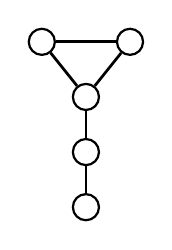
\begin{tikzpicture}[scale=\gscaling,auto,swap]

	% define the round nodes
	\foreach \pos/\name/\label in {
	  {(0,0)//1a},
	  {(-0.8,1)//2a},
	  {(0.8,1)//3a},
	  {(0,-1)//4a},
	  {(0,-2)//5a}}
	  \node[vertex2] (\label) at \pos {$\name$} ;

	%neighbouring graph
	      
	\path[hi, line width=1.0]  (1a)  -- (2a);
	\path[hi, line width=1.0]  (2a)  -- (3a);
	\path[hi, line width=1.0]  (1a)  -- (3a);
	\path[hi, line width=1.0]  (1a)  -- (4a);
	\path[hi, line width=1.0]  (4a)  -- (5a);

	
      \end{tikzpicture} & \Large{$G_{13}$}
    \end{tabular}
}

\newcommand{\gthirteencca}[1]{
    \begin{tabular}{>{\centering\bfseries}m{0.7in} >{\centering}m{0in}}	
      \begin{tikzpicture}[scale=\gscaling,auto,swap]

	% define the round nodes
	\foreach \pos/\name/\label in {
	  {(0,0)//1a},
	  {(-0.8,1)//2a},
	  {(0.8,1)//3a},
	  {(0,-1)//4a},
	  {(0,-2)//5a}}
	  \node[vertex3,draw=#1,fill=#1] (\label) at \pos {$\name$} ;

	%neighbouring graph
	      
	\path[hi, line width=1.0,draw=#1]  (1a)  -- (2a);
	\path[hi, line width=1.0,draw=#1]  (2a)  -- (3a);
	\path[hi, line width=1.0,draw=#1]  (1a)  -- (3a);
	\path[hi, line width=1.0,draw=#1]  (1a)  -- (4a);
	\path[hi, line width=1.0,draw=#1]  (4a)  -- (5a);

	
      \end{tikzpicture} \cellcolor{black} & \cellcolor{black}\textcolor{white}{\Large{$G_{13}$}}
    \end{tabular}
}


\newcommand{\gfourteen}{
    \begin{tabular}{>{\centering\bfseries}m{1in} >{\centering}m{0in}}	
      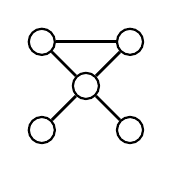
\begin{tikzpicture}[scale=\gscaling * 0.8,auto,swap]

	% define the round nodes
	\foreach \pos/\name/\label in {
	  {(0,0)//1a},
	  {(-1,1)//2a},
	  {(1,1)//3a},
	  {(-1,-1)//4a},
	  {(1,-1)//5a}}
	  \node[vertex2] (\label) at \pos {$\name$} ;

	%neighbouring graph
	      
	\path[hi, line width=1.0]  (1a)  -- (2a);
	\path[hi, line width=1.0]  (1a)  -- (3a);
	\path[hi, line width=1.0]  (2a)  -- (3a);
	\path[hi, line width=1.0]  (1a)  -- (4a);
	\path[hi, line width=1.0]  (1a)  -- (5a);

	
      \end{tikzpicture} & \Large{$G_{14}$}
    \end{tabular}
}



\newcommand{\gfourteencca}[1]{
    \begin{tabular}{>{\centering\bfseries}m{0.7in} >{\centering}m{0in}}	
      \begin{tikzpicture}[scale=\gscaling * 0.8,auto,swap]

	% define the round nodes
	\foreach \pos/\name/\label in {
	  {(0,0)//1a},
	  {(-1,1)//2a},
	  {(1,1)//3a},
	  {(-1,-1)//4a},
	  {(1,-1)//5a}}
	  \node[vertex3,draw=#1,fill=#1] (\label) at \pos {$\name$} ;

	%neighbouring graph
	      
	\path[hi, line width=1.0,draw=#1]  (1a)  -- (2a);
	\path[hi, line width=1.0,draw=#1]  (1a)  -- (3a);
	\path[hi, line width=1.0,draw=#1]  (2a)  -- (3a);
	\path[hi, line width=1.0,draw=#1]  (1a)  -- (4a);
	\path[hi, line width=1.0,draw=#1]  (1a)  -- (5a);

	
      \end{tikzpicture} \cellcolor{black} & \cellcolor{black}\textcolor{white}{\Large{$G_{14}$}}
    \end{tabular}
}

\newcommand{\gfifteen}{
    \begin{tabular}{>{\centering\bfseries}m{1in} >{\centering}m{0in}}	
      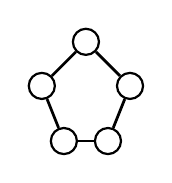
\begin{tikzpicture}[scale=\gscaling,auto,swap]

	% define the round nodes
	\foreach \pos/\name/\label in {
	  {(0,1)//1a},
	  {(-0.8,0.2)//2a},
	  {(-0.4,-0.8)//3a},
	  {(0.4,-0.8)//4a},
	  {(0.8,0.2)//5a}}
	  \node[vertex2] (\label) at \pos {$\name$} ;

	%neighbouring graph
	      
	\path[hi, line width=1.0]  (1a)  -- (2a);
	\path[hi, line width=1.0]  (2a)  -- (3a);
	\path[hi, line width=1.0]  (3a)  -- (4a);
	\path[hi, line width=1.0]  (4a)  -- (5a);
	\path[hi, line width=1.0]  (5a)  -- (1a);

	
      \end{tikzpicture} & \Large{$G_{15}$}
    \end{tabular}
}

\newcommand{\gfifteencca}[1]{
    \begin{tabular}{>{\centering\bfseries}m{0.7in} >{\centering}m{0in}}	
      \begin{tikzpicture}[scale=\gscaling,auto,swap]

	% define the round nodes
	\foreach \pos/\name/\label in {
	  {(0,1)//1a},
	  {(-0.8,0.2)//2a},
	  {(-0.4,-0.8)//3a},
	  {(0.4,-0.8)//4a},
	  {(0.8,0.2)//5a}}
	  \node[vertex2,draw=#1,fill=#1] (\label) at \pos {$\name$} ;

	%neighbouring graph
	      
	\path[hi, line width=1.0,draw=#1]  (1a)  -- (2a);
	\path[hi, line width=1.0,draw=#1]  (2a)  -- (3a);
	\path[hi, line width=1.0,draw=#1]  (3a)  -- (4a);
	\path[hi, line width=1.0,draw=#1]  (4a)  -- (5a);
	\path[hi, line width=1.0,draw=#1]  (5a)  -- (1a);

	
      \end{tikzpicture} \cellcolor{black} & \cellcolor{black}\textcolor{white}{\Large{$G_{15}$}}
    \end{tabular}
}


\newcommand{\gsixteen}{
    \begin{tabular}{>{\centering\bfseries}m{1in} >{\centering}m{0in}}	
      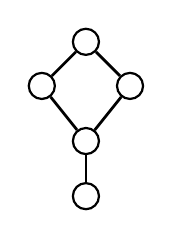
\begin{tikzpicture}[scale=\gscaling,auto,swap]

	% define the round nodes
	\foreach \pos/\name/\label in {
	  {(0,0)//1a},
	  {(-0.8,1)//2a},
	  {(0.8,1)//3a},
	  {(0,-1)//4a},
	  {(0,1.8)//5a}}
	  \node[vertex2] (\label) at \pos {$\name$} ;

	%neighbouring graph
	      
	\path[hi, line width=1.0]  (1a)  -- (2a);
	\path[hi, line width=1.0]  (2a)  -- (5a);
	\path[hi, line width=1.0]  (3a)  -- (5a);
	\path[hi, line width=1.0]  (1a)  -- (3a);
	\path[hi, line width=1.0]  (1a)  -- (4a);


      \end{tikzpicture} & \Large{$G_{16}$}
    \end{tabular}
}



\newcommand{\gsixteencca}[1]{
    \begin{tabular}{>{\centering\bfseries}m{0.7in} >{\centering}m{0in}}	
      \begin{tikzpicture}[scale=\gscaling,auto,swap]

	% define the round nodes
	\foreach \pos/\name/\label in {
	  {(0,0)//1a},
	  {(-0.8,1)//2a},
	  {(0.8,1)//3a},
	  {(0,-1)//4a},
	  {(0,1.8)//5a}}
	  \node[vertex3,draw=#1,fill=#1] (\label) at \pos {$\name$} ;

	%neighbouring graph
	      
	\path[hi, line width=1.0,draw=#1]  (1a)  -- (2a);
	\path[hi, line width=1.0,draw=#1]  (2a)  -- (5a);
	\path[hi, line width=1.0,draw=#1]  (3a)  -- (5a);
	\path[hi, line width=1.0,draw=#1]  (1a)  -- (3a);
	\path[hi, line width=1.0,draw=#1]  (1a)  -- (4a);


      \end{tikzpicture} \cellcolor{black} & \cellcolor{black}\textcolor{white}{\Large{$G_{16}$}}
    \end{tabular}
}

\newcommand{\gtwenty}{
    \begin{tabular}{>{\centering\bfseries}m{1in} >{\centering}m{0in}}	
      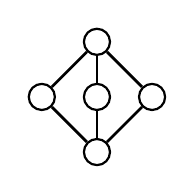
\begin{tikzpicture}[scale=\gscaling,auto,swap]

	% define the round nodes
	\foreach \pos/\name/\label in {
	  {(-1.0,0)//1a},
	  {(0,0)//2a},
	  {(1,0)//3a},
	  {(0,1)//4a},
	  {(0,-1)//5a}}
	  \node[vertex2] (\label) at \pos {$\name$} ;

	%neighbouring graph
	      
	\path[hi, line width=1.0]  (1a)  -- (4a);
	\path[hi, line width=1.0]  (2a)  -- (4a);
	\path[hi, line width=1.0]  (3a)  -- (4a);
	\path[hi, line width=1.0]  (1a)  -- (5a);
	\path[hi, line width=1.0]  (2a)  -- (5a);
	\path[hi, line width=1.0]  (3a)  -- (5a);

	
      \end{tikzpicture} & \Large{$G_{20}$}
    \end{tabular}
}

\newcommand{\gtwentycca}[1]{
    \begin{tabular}{>{\centering\bfseries}m{0.7in} >{\centering}m{0in}}	
      \begin{tikzpicture}[scale=\gscaling,auto,swap]

	% define the round nodes
	\foreach \pos/\name/\label in {
	  {(-1.0,0)//1a},
	  {(0,0)//2a},
	  {(1,0)//3a},
	  {(0,1)//4a},
	  {(0,-1)//5a}}
	  \node[vertex2,draw=#1,fill=#1] (\label) at \pos {$\name$} ;

	%neighbouring graph
	      
	\path[hi, line width=1.0,draw=#1]  (1a)  -- (4a);
	\path[hi, line width=1.0,draw=#1]  (2a)  -- (4a);
	\path[hi, line width=1.0,draw=#1]  (3a)  -- (4a);
	\path[hi, line width=1.0,draw=#1]  (1a)  -- (5a);
	\path[hi, line width=1.0,draw=#1]  (2a)  -- (5a);
	\path[hi, line width=1.0,draw=#1]  (3a)  -- (5a);

	
      \end{tikzpicture} \cellcolor{black} & \cellcolor{black}\textcolor{white}{\Large{$G_{20}$}}
    \end{tabular}
}


\newcommand{\gtwentyone}{
    \begin{tabular}{>{\centering\bfseries}m{1in} >{\centering}m{0in}}	
      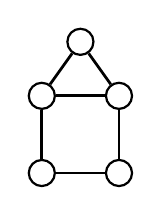
\begin{tikzpicture}[scale=\gscaling * 1.4,auto,swap]

	% define the round nodes
	\foreach \pos/\name/\label in {
	  {(0,0)//1a},
	  {(1,0)//2a},
	  {(0.5,0.7)//3a},
	  {(0,-1)//4a},
	  {(1,-1)//5a}}
	  \node[vertex2] (\label) at \pos {$\name$} ;

	%neighbouring graph
	      
	\path[hi, line width=1.0]  (1a)  -- (2a);
	\path[hi, line width=1.0]  (1a)  -- (3a);
	\path[hi, line width=1.0]  (2a)  -- (3a);
	\path[hi, line width=1.0]  (1a)  -- (4a);
	\path[hi, line width=1.0]  (2a)  -- (5a);
	\path[hi, line width=1.0]  (4a)  -- (5a);

	
      \end{tikzpicture} & \Large{$G_{21}$}
    \end{tabular}
}


\newcommand{\gtwentytwo}{
    \begin{tabular}{>{\centering\bfseries}m{1in} >{\centering}m{0in}}	
      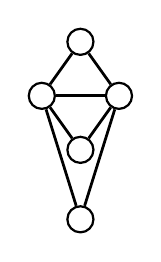
\begin{tikzpicture}[scale=\gscaling * 1.4,auto,swap]

	% define the round nodes
	\foreach \pos/\name/\label in {
	  {(0,0)//1a},
	  {(1,0)//2a},
	  {(0.5,0.7)//3a},
	  {(0.5,-0.7)//4a},
	  {(0.5,-1.6)//5a}}
	  \node[vertex2] (\label) at \pos {$\name$} ;

	%neighbouring graph

	\path[hi, line width=1.0]  (1a)  -- (2a);	
	\path[hi, line width=1.0]  (1a)  -- (3a);
	\path[hi, line width=1.0]  (1a)  -- (4a);
	\path[hi, line width=1.0]  (1a)  -- (5a);
	\path[hi, line width=1.0]  (2a)  -- (3a);
	\path[hi, line width=1.0]  (2a)  -- (4a);
	\path[hi, line width=1.0]  (2a)  -- (5a);

	
      \end{tikzpicture} & \Large{$G_{22}$}
    \end{tabular}
}


\newcommand{\gtwentythree}{
    \begin{tabular}{>{\centering\bfseries}m{1in} >{\centering}m{0in}}	
      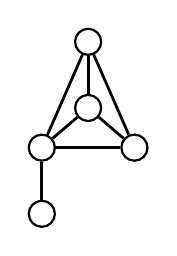
\begin{tikzpicture}[scale=\gscaling * 1.2,auto,swap]

	% define the round nodes
	\foreach \pos/\name/\label in {
	  {(0,0)//1a},
	  {(-0.7,-0.6)//2a},
	  {(0.7,-0.6)//3a},
	  {(0,1)//4a},
	  {(-0.7,-1.6)//5a}}
	  \node[vertex2] (\label) at \pos {$\name$} ;

	%neighbouring graph
	      
	\path[hi, line width=1.0]  (1a)  -- (2a);
	\path[hi, line width=1.0]  (1a)  -- (3a);
	\path[hi, line width=1.0]  (1a)  -- (4a);
	\path[hi, line width=1.0]  (2a)  -- (3a);
	\path[hi, line width=1.0]  (2a)  -- (4a);
	\path[hi, line width=1.0]  (3a)  -- (4a);
	\path[hi, line width=1.0]  (2a)  -- (5a);
	
      \end{tikzpicture} & \Large{$G_{23}$}
    \end{tabular}
}


\newcommand{\gtwentyfour}{
    \begin{tabular}{>{\centering\bfseries}m{1in} >{\centering}m{0in}}	
      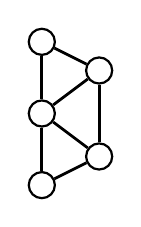
\begin{tikzpicture}[scale=\gscaling * 1.3,auto,swap]

	% define the round nodes
	\foreach \pos/\name/\label in {
	  {(0,0)//1a},
	  {(0,1)//2a},
	  {(0.8,0.6)//3a},
	  {(0.8,-0.6)//4a},
	  {(0,-1)//5a}}
	  \node[vertex2] (\label) at \pos {$\name$} ;

	%neighbouring graph

	\path[hi, line width=1.0]  (1a)  -- (2a);	
	\path[hi, line width=1.0]  (1a)  -- (3a);
	\path[hi, line width=1.0]  (1a)  -- (4a);
	\path[hi, line width=1.0]  (1a)  -- (5a);
	\path[hi, line width=1.0]  (2a)  -- (3a);
	\path[hi, line width=1.0]  (3a)  -- (4a);
	\path[hi, line width=1.0]  (4a)  -- (5a);

	
      \end{tikzpicture} & \Large{$G_{24}$}
    \end{tabular}
}


\newcommand{\gtwentyfive}{
    \begin{tabular}{>{\centering\bfseries}m{1in} >{\centering}m{0in}}	
      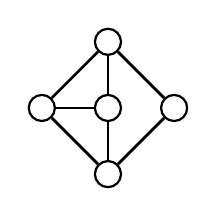
\begin{tikzpicture}[scale=\gscaling * 1.2,auto,swap]

	% define the round nodes
	\foreach \pos/\name/\label in {
	  {(-1.0,0)//1a},
	  {(0,0)//2a},
	  {(1,0)//3a},
	  {(0,1)//4a},
	  {(0,-1)//5a}}
	  \node[vertex2] (\label) at \pos {$\name$} ;

	%neighbouring graph

	\path[hi, line width=1.0]  (1a)  -- (2a);	
	\path[hi, line width=1.0]  (1a)  -- (4a);
	\path[hi, line width=1.0]  (2a)  -- (4a);
	\path[hi, line width=1.0]  (3a)  -- (4a);
	\path[hi, line width=1.0]  (1a)  -- (5a);
	\path[hi, line width=1.0]  (2a)  -- (5a);
	\path[hi, line width=1.0]  (3a)  -- (5a);

	
      \end{tikzpicture} & \Large{$G_{25}$}
    \end{tabular}
}


\newcommand{\gtwentysix}{
    \begin{tabular}{>{\centering\bfseries}m{1in} >{\centering}m{0in}}	
      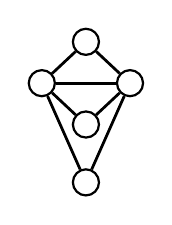
\begin{tikzpicture}[scale=\gscaling * 1.0,auto,swap]

	% define the round nodes
	\foreach \pos/\name/\label in {
	  {(-0.8,0)//1a},
	  {(0.8,0)//2a},
	  {(0,0.75)//3a},
	  {(0,-0.75)//4a},
	  {(0,-1.8)//5a}}
	  \node[vertex2] (\label) at \pos {$\name$} ;

	%neighbouring graph

	\path[hi, line width=1.0]  (1a)  -- (2a);	
	\path[hi, line width=1.0]  (1a)  -- (3a);
	\path[hi, line width=1.0]  (1a)  -- (4a);
	\path[hi, line width=1.0]  (1a)  -- (5a);
	\path[hi, line width=1.0]  (2a)  -- (3a);
	\path[hi, line width=1.0]  (2a)  -- (4a);
	\path[hi, line width=1.0]  (2a)  -- (5a);

	
      \end{tikzpicture} & \Large{$G_{26}$}
    \end{tabular}
}



\newcommand{\gtwentyseven}{
    \begin{tabular}{>{\centering\bfseries}m{1in} >{\centering}m{0in}}	
      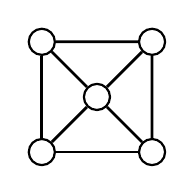
\begin{tikzpicture}[scale=\gscaling*2,auto,swap]

	% define the round nodes
	\foreach \pos/\name/\label in {
	  {(0,0)//1a},
	  {(0,1)//2a},
	  {(1,1)//3a},
	  {(1,0)//4a},
	  {(0.5,0.5)//5a}}
	  \node[vertex2] (\label) at \pos {$\name$} ;

	%neighbouring graph
	      
	\path[hi, line width=1.0]  (1a)  -- (2a);
	\path[hi, line width=1.0]  (2a)  -- (3a);
	\path[hi, line width=1.0]  (3a)  -- (4a);
	\path[hi, line width=1.0]  (1a)  -- (4a);
	\path[hi, line width=1.0]  (5a)  -- (2a);
	\path[hi, line width=1.0]  (5a)  -- (3a);
	\path[hi, line width=1.0]  (5a)  -- (4a);
	\path[hi, line width=1.0]  (5a)  -- (1a);

	
      \end{tikzpicture} & \Large{$G_{27}$}
    \end{tabular}
}


\newcommand{\gtwentynine}{
    \begin{tabular}{>{\centering\bfseries}m{1in} >{\centering}m{0in}}	
      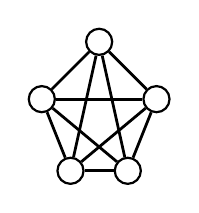
\begin{tikzpicture}[scale=\gscaling * 1.3,auto,swap]

	% define the round nodes
	\foreach \pos/\name/\label in {
	  {(0,1)//1a},
	  {(-0.8,0.2)//2a},
	  {(-0.4,-0.8)//3a},
	  {(0.4,-0.8)//4a},
	  {(0.8,0.2)//5a}}
	  \node[vertex2] (\label) at \pos {$\name$} ;

	%neighbouring graph
	      
	\path[hi, line width=1.0]  (1a)  -- (2a);
	\path[hi, line width=1.0]  (1a)  -- (3a);
	\path[hi, line width=1.0]  (1a)  -- (4a);
	\path[hi, line width=1.0]  (1a)  -- (5a);
	\path[hi, line width=1.0]  (2a)  -- (3a);
	\path[hi, line width=1.0]  (2a)  -- (4a);
	\path[hi, line width=1.0]  (2a)  -- (5a);
	\path[hi, line width=1.0]  (3a)  -- (4a);
	\path[hi, line width=1.0]  (3a)  -- (5a);
	\path[hi, line width=1.0]  (4a)  -- (5a);


	
      \end{tikzpicture} & \Large{$G_{29}$}
    \end{tabular}
}

\newcommand{\gtwentyninepic}{
      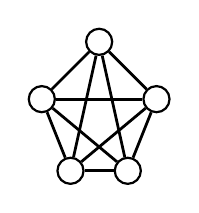
\begin{tikzpicture}[scale=\gscaling * 1.3,auto,swap]

	% define the round nodes
	\foreach \pos/\name/\label in {
	  {(0,1)//1a},
	  {(-0.8,0.2)//2a},
	  {(-0.4,-0.8)//3a},
	  {(0.4,-0.8)//4a},
	  {(0.8,0.2)//5a}}
	  \node[vertex2] (\label) at \pos {$\name$} ;

	%neighbouring graph
	      
	\path[hi, line width=1.0]  (1a)  -- (2a);
	\path[hi, line width=1.0]  (1a)  -- (3a);
	\path[hi, line width=1.0]  (1a)  -- (4a);
	\path[hi, line width=1.0]  (1a)  -- (5a);
	\path[hi, line width=1.0]  (2a)  -- (3a);
	\path[hi, line width=1.0]  (2a)  -- (4a);
	\path[hi, line width=1.0]  (2a)  -- (5a);
	\path[hi, line width=1.0]  (3a)  -- (4a);
	\path[hi, line width=1.0]  (3a)  -- (5a);
	\path[hi, line width=1.0]  (4a)  -- (5a);


	
      \end{tikzpicture}
}


\newcommand{\gtwentyninecca}[1]{
    \begin{tabular}{>{\centering\bfseries}m{0.7in} >{\centering}m{0in}}	
      \cellcolor{black}\begin{tikzpicture}[scale=\gscaling * 1.3,auto,swap]

	% define the round nodes
	\foreach \pos/\name/\label in {
	  {(0,1)//1a},
	  {(-0.8,0.2)//2a},
	  {(-0.4,-0.8)//3a},
	  {(0.4,-0.8)//4a},
	  {(0.8,0.2)//5a}}
	  \node[vertex3,draw=#1,fill=#1] (\label) at \pos {$\name$} ;

	%neighbouring graph
	      
	\path[hi, line width=1.0,draw=#1]  (1a)  -- (2a);
	\path[hi, line width=1.0,draw=#1]  (1a)  -- (3a);
	\path[hi, line width=1.0,draw=#1]  (1a)  -- (4a);
	\path[hi, line width=1.0,draw=#1]  (1a)  -- (5a);
	\path[hi, line width=1.0,draw=#1]  (2a)  -- (3a);
	\path[hi, line width=1.0,draw=#1]  (2a)  -- (4a);
	\path[hi, line width=1.0,draw=#1]  (2a)  -- (5a);
	\path[hi, line width=1.0,draw=#1]  (3a)  -- (4a);
	\path[hi, line width=1.0,draw=#1]  (3a)  -- (5a);
	\path[hi, line width=1.0,draw=#1]  (4a)  -- (5a);


	
      \end{tikzpicture} & \cellcolor{black}\textcolor{white}{\Large{$G_{29}$}}
    \end{tabular}
}


\newcommand{\gdots}{
    \begin{tabular}{>{\centering\bfseries}m{-2in} >{\centering}m{0in}}	
    \vdots & 
    \end{tabular}
}


\definecolor{ccacol0}{rgb}{0.00,1.00,0}%1
\definecolor{ccacol1}{rgb}{0.20,1.00,0}%0.8 
\definecolor{ccacol2}{rgb}{0.40,1.00,0}%0.6
\definecolor{ccacol3}{rgb}{0.60,1.00,0}%0.4
\definecolor{ccacol4}{rgb}{0.80,1.00,0}%0.2
\definecolor{ccacol5}{rgb}{1.00,1.00,0}%0.0
\definecolor{ccacol6}{rgb}{1.00,0.80,0}%-0.2
\definecolor{ccacol7}{rgb}{1.00,0.60,0}%-0.4
\definecolor{ccacol8}{rgb}{1.00,0.40,0}%-0.6
\definecolor{ccacol9}{rgb}{1.00,0.20,0}%-0.8
\definecolor{ccacol10}{rgb}{1.00,0.00,0}%-1


\newcommand{\ccafigscale}{0.6}

\newcommand{\ccafigscaleppi}{0.55}

\begin{document}

\title[On a New Signature that quantifies Topological Structure] % (optional, only for long titles)
{On a New Signature that quantifies Topological Structure in Biological and Economic networks}
% \subtitle{Evidence from India}
\author[Razvan Valentin Marinescu] % (optional, for multiple authors)
{Razvan Valentin Marinescu}
\institute[Imperial College London] % (optional)
{
%   \inst{1}%
  Department of Computing\\
  Imperial College London
}
\date{23 June 2014} % (optional)
\subject{Computer Science}

\frame{\titlepage}

\begin{frame}
   \frametitle{Neighbourhood comparison using the clustering coefficient}
  \begin{minipage}{\textwidth}
  \begin{center}
  %A
  \noindent\begin{minipage}[b]{.45\textwidth}
  \centering
  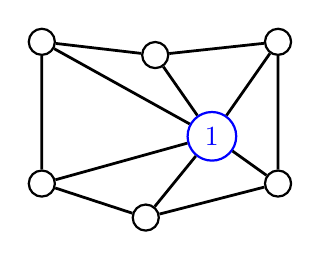
\begin{tikzpicture}[scale=1.2,auto,swap]

  %   \draw (-2,0) ellipse (0.85cm and 1.8cm);
  %   \node[upper left] at (current bounding box.north east) {\textbf{$S_1$}};	
    
    % define the round nodes
    \node[vertex,blue] (1a) at (0.3,0) {$1$};
    
      \foreach \pos/\name/\label in {
	{(1,-0.5)//2a},
	{(1,1)//3a},
	{(-0.3,0.86)//4a},
	{(-1.5,1)//5a}, 
	{(-1.5,-0.5)//6a},
	{(-0.4,-0.86)//7a}}
	\node[vertex] (\label) at \pos {$\name$} ;

  %     \node[upper left,inner sep=0] (src_lab) at (-0.5,0.75) {\begin{tabular}{r} source\\ node \end{tabular}};
  %     \draw[->, thick]  (src_lab)  -- (1a) {}; 
      
    %neighbouring graph
	  
    \path[hi, line width=1.0]  (5a)  -- (6a);
    \path[hi, line width=1.0]  (6a)  -- (7a);
    \path[hi, line width=1.0]  (7a)  -- (2a);
    \path[hi, line width=1.0]  (2a)  -- (3a);
    \path[hi, line width=1.0]  (3a)  -- (4a);
    \path[hi, line width=1.0]  (4a)  -- (5a);
  %   \path[hi, line width=1.0]  (6a)  -- (2a);
    
    % rest of edges, dotted

    \path[hi, line width=1.0]  (1a)  -- (2a);
    \path[hi, line width=1.0]  (1a)  -- (3a);
    \path[hi, line width=1.0]  (1a)  -- (4a);
    \path[hi, line width=1.0]  (1a)  -- (5a);
    \path[hi, line width=1.0]  (1a)  -- (6a);
    \path[hi, line width=1.0]  (1a)  -- (7a);
    
  \end{tikzpicture}
  \captionof{figure}{Graph 1}
  \end{minipage} 
  \hfill
  \begin{minipage}[b]{.45\textwidth}
    \centering
    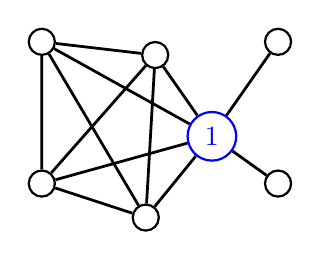
\begin{tikzpicture}[scale=1.2,auto,swap]

    %   \draw (-2,0) ellipse (0.85cm and 1.8cm);
    %   \node[upper left] at (current bounding box.north east) {\textbf{$S_1$}};	
      
      % define the round nodes
      \node[vertex,blue] (1a) at (0.3,0) {$1$};
      
      \foreach \pos/\name/\label in {
	{(1,-0.5)//2a},
	{(1,1)//3a},
	{(-0.3,0.86)//4a},
	{(-1.5,1)//5a}, 
	{(-1.5,-0.5)//6a},
	{(-0.4,-0.86)//7a}}
	\node[vertex] (\label) at \pos {$\name$} ;

	
      %neighbouring graph
	    
      \path[hi, line width=1.0]  (5a)  -- (4a);
      \path[hi, line width=1.0]  (4a)  -- (6a);
      \path[hi, line width=1.0]  (6a)  -- (5a);
      \path[hi, line width=1.0]  (7a)  -- (6a);
      \path[hi, line width=1.0]  (4a)  -- (7a);
      \path[hi, line width=1.0]  (7a)  -- (5a);
    %   \path[hi, line width=1.0]  (6a)  -- (2a);
      
      % edges from 1 to rest

      \path[hi, line width=1.0]  (1a)  -- (2a);
      \path[hi, line width=1.0]  (1a)  -- (3a);
      \path[hi, line width=1.0]  (1a)  -- (4a);
      \path[hi, line width=1.0]  (1a)  -- (5a);
      \path[hi, line width=1.0]  (1a)  -- (6a);
      \path[hi, line width=1.0]  (1a)  -- (7a);
      
    \end{tikzpicture}
    \captionof{figure}{Graph 2}
  \end{minipage}
  \end{center}
  \end{minipage}


  
\end{frame}


\newcommand{\graphone}[1]{
\begin{minipage}[b]{.45\textwidth}
  \centering
  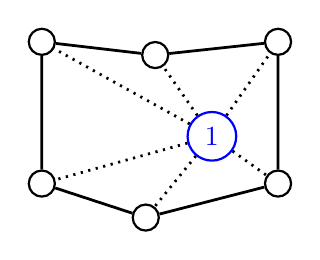
\begin{tikzpicture}[scale=1.2,auto,swap]

  %   \draw (-2,0) ellipse (0.85cm and 1.8cm);
  %   \node[upper left] at (current bounding box.north east) {\textbf{$S_1$}};	
    
    % define the round nodes
    \node[vertex,blue] (1a) at (0.3,0) {$1$};
    
      \foreach \pos/\name/\label in {
	{(1,-0.5)//2a},
	{(1,1)//3a},
	{(-0.3,0.86)//4a},
	{(-1.5,1)//5a}, 
	{(-1.5,-0.5)//6a},
	{(-0.4,-0.86)//7a}}
	\node[vertex] (\label) at \pos {$\name$} ;

  %     \node[upper left,inner sep=0] (src_lab) at (-0.5,0.75) {\begin{tabular}{r} source\\ node \end{tabular}};
  %     \draw[->, thick]  (src_lab)  -- (1a) {}; 
      
    %neighbouring graph
	  
    \path[hi, line width=1.0]  (5a)  -- (6a);
    \path[hi, line width=1.0]  (6a)  -- (7a);
    \path[hi, line width=1.0]  (7a)  -- (2a);
    \path[hi, line width=1.0]  (2a)  -- (3a);
    \path[hi, line width=1.0]  (3a)  -- (4a);
    \path[hi, line width=1.0]  (4a)  -- (5a);
  %   \path[hi, line width=1.0]  (6a)  -- (2a);
    
    % rest of edges, dotted

    \path[lo, line width=1.0]  (1a)  -- (2a);
    \path[lo, line width=1.0]  (1a)  -- (3a);
    \path[lo, line width=1.0]  (1a)  -- (4a);
    \path[lo, line width=1.0]  (1a)  -- (5a);
    \path[lo, line width=1.0]  (1a)  -- (6a);
    \path[lo, line width=1.0]  (1a)  -- (7a);
    
  \end{tikzpicture}
  \captionof{figure}{#1}
  \end{minipage} 
}

\newcommand{\graphtwo}[1]{
\begin{minipage}[b]{.45\textwidth}
    \centering
    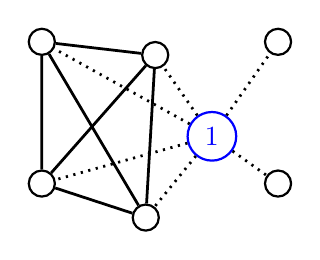
\begin{tikzpicture}[scale=1.2,auto,swap]

    %   \draw (-2,0) ellipse (0.85cm and 1.8cm);
    %   \node[upper left] at (current bounding box.north east) {\textbf{$S_1$}};	
      
      % define the round nodes
      \node[vertex,blue] (1a) at (0.3,0) {$1$};
      
      \foreach \pos/\name/\label in {
	{(1,-0.5)//2a},
	{(1,1)//3a},
	{(-0.3,0.86)//4a},
	{(-1.5,1)//5a}, 
	{(-1.5,-0.5)//6a},
	{(-0.4,-0.86)//7a}}
	\node[vertex] (\label) at \pos {$\name$} ;

	
      %neighbouring graph
	    
      \path[hi, line width=1.0]  (5a)  -- (4a);
      \path[hi, line width=1.0]  (4a)  -- (6a);
      \path[hi, line width=1.0]  (6a)  -- (5a);
      \path[hi, line width=1.0]  (7a)  -- (6a);
      \path[hi, line width=1.0]  (4a)  -- (7a);
      \path[hi, line width=1.0]  (7a)  -- (5a);
    %   \path[hi, line width=1.0]  (6a)  -- (2a);
      
      % edges from 1 to rest

    \path[lo, line width=1.0]  (1a)  -- (2a);
    \path[lo, line width=1.0]  (1a)  -- (3a);
    \path[lo, line width=1.0]  (1a)  -- (4a);
    \path[lo, line width=1.0]  (1a)  -- (5a);
    \path[lo, line width=1.0]  (1a)  -- (6a);
    \path[lo, line width=1.0]  (1a)  -- (7a);
      
    \end{tikzpicture}
  \captionof{figure}{#1}
  \end{minipage}
}

\begin{frame}
  \frametitle{Neighbourhood comparison using the clustering coefficient}
  
  \begin{minipage}{\textwidth}
  \begin{center}
  %A
  \noindent
  \graphone{Clustering coefficient: 0.4}
  \hfill
  \graphtwo{Clustering coefficient: 0.4}
  \end{center}
  \end{minipage}

  \vfill
  \begin{itemize}
   \item Problem: the clustering coefficient cannot distinguish between the two graphs \dots
   \item Solution: generalise the clustering coefficient!
  \end{itemize}

\end{frame}

% GCV + graphlets image
\begin{frame}
  \frametitle{Clustering coefficient generalisation}
  
  \begin{itemize}
   \item \textbf{Graphlet Cluster Vector} (GCV) - generalises the clustering coefficient. 
   \item $GCV = \{F_1, F_2, \dots, F_{29}\}$
  \end{itemize}
  
  \vfill
  

\begin{figure}
 \centering
 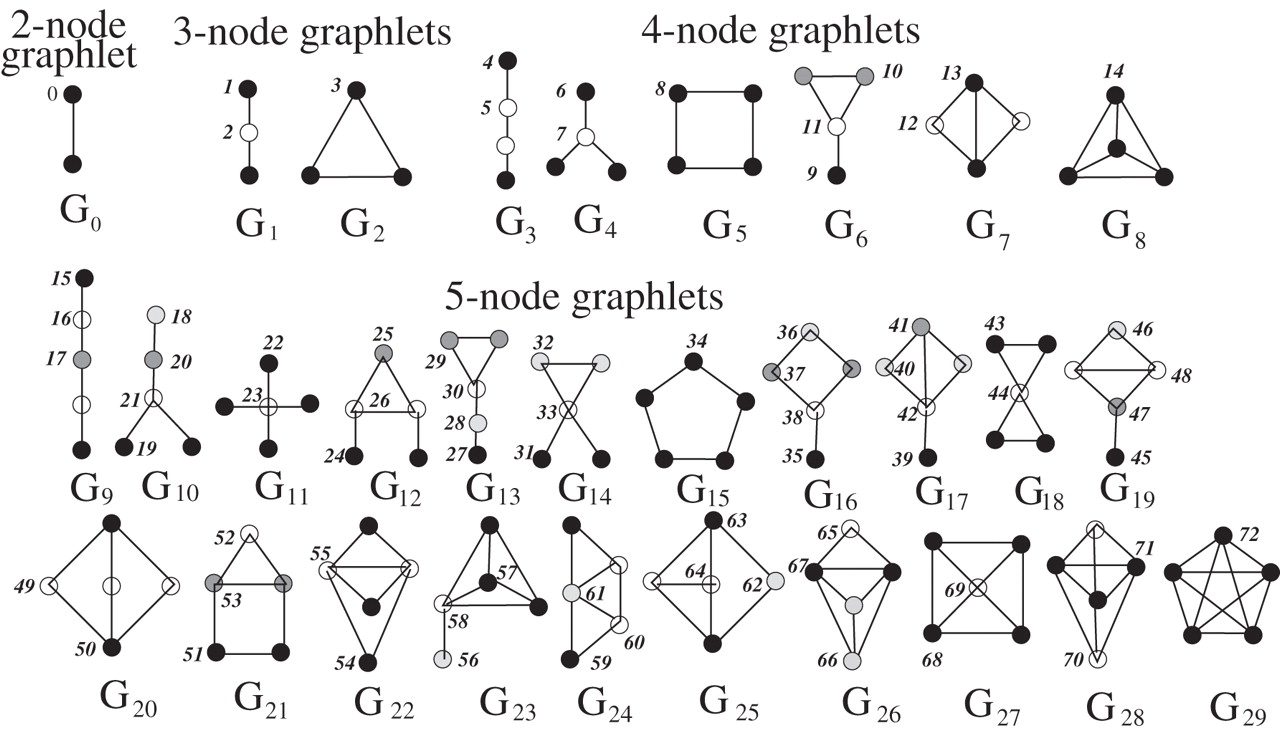
\includegraphics[scale=0.20]{../report_imperial/images/graphlets.jpg} 
\end{figure}

\end{frame}

% \begin{frame}
% \frametitle{GCV example}
%  
%  \begin{figure} 
% \centering
% \begin{tikzpicture}[scale=1.0,auto,swap]
% 
%   \draw (-2,0) ellipse (0.99cm and 1.97cm);
%   \node[upper left] at (current bounding box.north east) {\textbf{$S_1$}};	
%   
%   % define the round nodes
%   \node[vertex,blue] (1a) at (-3.75877048314363,0) {$1$};
%   
%   \foreach \pos/\name/\label in {
%     {(-2.0,1.46)/2/2a},
%     {(-2.5,0.5)/3/3a},
%     {(-1.5,-0.5)/4/4a},
%     {(-2.0,-1.46)/5/5a},
%     {(0.5,-0.46)/6/6a}}
%     \node[vertex] (\label) at \pos {$\name$} ;
% 
%     \node[upper left,inner sep=0] (src_lab) at (-5.0,1.2) {\rowcolors{1}{}{}\begin{tabular}{r} source\\ node \end{tabular}};
%     \draw[->, thick]  (src_lab)  -- (1a) {}; 
%     
%   %neighbouring graph
% 	
%   \path[hi, line width=1.0]  (4a)  -- (3a);
%   \path[hi, line width=1.0]  (2a)  -- (4a);
%   \path[hi, line width=1.0]  (5a)  -- (4a);
%   
%   % rest of edges, dotted
% 
%   \path[lo, line width=1.0]  (1a)  -- (2a);
%   \path[lo, line width=1.0]  (1a)  -- (3a);
%   \path[lo, line width=1.0]  (1a)  -- (4a);
%   \path[lo, line width=1.0]  (1a)  -- (5a);
%   \path[lo, line width=1.0]  (6a)  -- (5a);
% \end{tikzpicture}
% \caption{GCV(1) = $(3,3,0,1,0,0,0,...)$}
% \end{figure}
%  
% \end{frame}



% GCV on the 2 graphs
\begin{frame}
  \frametitle{Comparison using the GCV}
  \begin{minipage}{\textwidth}
  \begin{center}
  %A
  \noindent
  \graphone{$GCV = \{6,0,6,0,0,0,0,0, \dots \}$}
  \hfill
  \graphtwo{$GCV = \{0,4,0,0,0,0,0,1, \dots \}$}
  \end{center}
  \end{minipage}  
  
%   \hilight{TODO: Add graphlet images pointing to the elements of the GCV}
  
\end{frame}

\begin{frame}
 \frametitle{Presentation outline}
 
 \begin{itemize}
  \item \textcolor{red}{GCV Implementation} \vfill
  \item Applications \vfill
  
  \begin{figure}
    \hspace{-3em}
    \begin{tikzpicture}[scale=0.7,auto,swap]


    \node[inner sep=0pt] (trade) at (-5.5, 0.5) {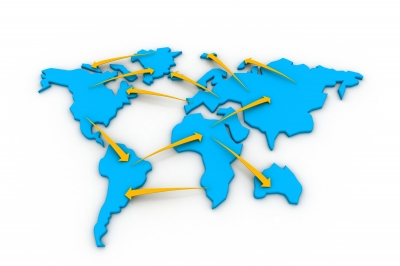
\includegraphics[width=0.33\textwidth]{images/world_trade_net.jpg}};
    \node[inner sep=0pt] (ppi) at (0, 0.0) {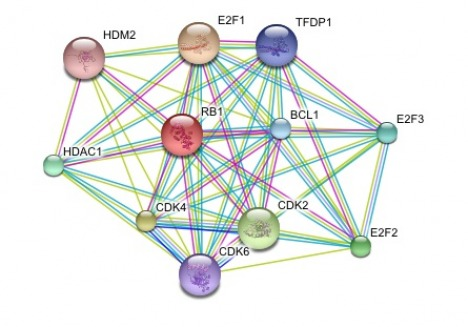
\includegraphics[width=0.33\textwidth]{images/protein_network.jpg}};
    \node[inner sep=0pt] (meta) at (5.5, 0.0) {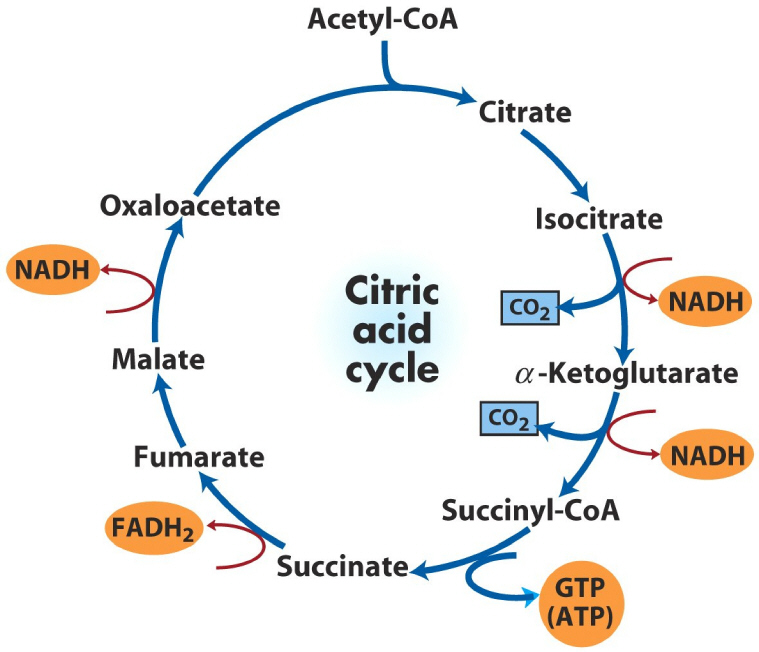
\includegraphics[scale=0.5]{images/metabolic_net.jpg}};

    \node[inner sep=0pt] (trade_label) at (-5.5,3) {\begin{tabular}{c} World Trade\\ networks \end{tabular}};
    \node[inner sep=0pt] (ppi_label) at (0,3) {\begin{tabular}{c} Protein Interaction\\ networks \end{tabular}};
    \node[inner sep=0pt] (meta_label) at (5.5,3) {\begin{tabular}{c} Metabolic\\ networks \end{tabular} };

    \end{tikzpicture}
  \end{figure}
  \item Evaluation on random graphs clustering \vfill
 \end{itemize}
 
\end{frame}


\begin{frame}
  \frametitle{Implementation}
  
  \begin{itemize}
   \item programming language: \lstinline|C++| \vfill
   \item we leveraged code (\lstinline|ncount.cpp|) that was computing a similar signature, called the GDV \vfill
   \item graph was represented by a complex data structure containing both: \vfill
   \begin{itemize}
    \item an adjacency matrix \vfill
    \item an adjacency list \vfill
   \end{itemize}
  \end{itemize}

%   \hilight{TODO: add some diagrams here instead of text}
  
\end{frame}


\begin{frame}
 \frametitle{Parallelisation}
   
  \begin{itemize}
   \item allowed us to run the GCV computation on large networks such as the PPI networks (11,000 nodes)
  \end{itemize}
  
 %%%%%%%%%% Parallelisation process %%%%%%%%%%%%%

\begin{figure}[H]
  \begin{center}
  \begin{tikzpicture}[scale=0.7,auto,swap,post/.style={->,shorten >=3pt,>=stealth',thick}, every node/.style={scale=0.7}]


    \node[inner sep=0pt] (network) at (-9.0, 0.0) {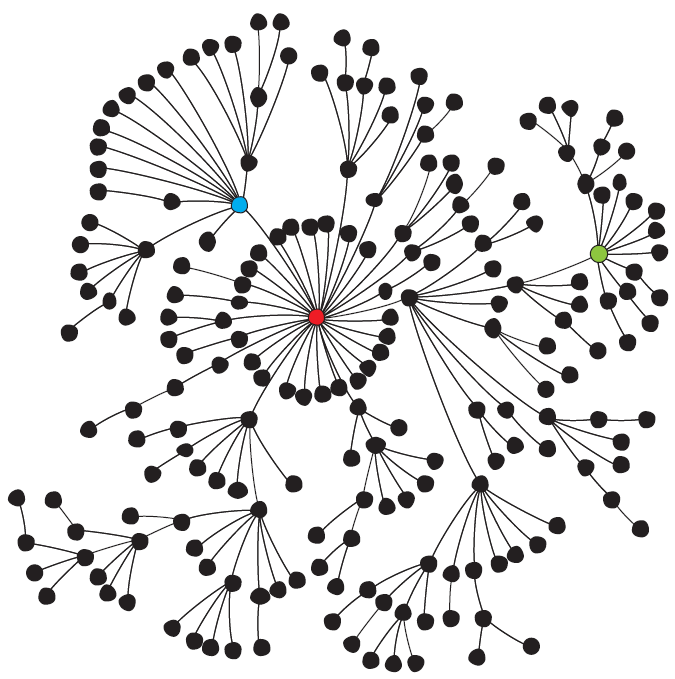
\includegraphics[width=0.4\textwidth]{../report_imperial/images/scale-free-network.png}};

    \node (proc1) at (-3.5,2) [draw,thick,minimum width=2cm,minimum height=1cm,rounded corners=10pt] {Process 1};
    \node (proc2) at (-3.5,-2) [draw,thick,minimum width=2cm,minimum height=1cm,rounded corners=10pt] {Process $n$};

    \node (file1) at (0,2) [draw,thick,minimum width=2cm,minimum height=1cm,rounded corners=10pt] {GCV list 1};
    \node (file2) at (0,-2) [draw,thick,minimum width=2cm,minimum height=1cm,rounded corners=10pt] {GCV list $n$};
    
    \node (file_final) at (3,0) [draw,thick,minimum width=2cm,minimum height=1cm,rounded corners=10pt] {Final GCV list};
    
    \draw node[circle, minimum size=2cm, red, fill=red, fill opacity=0.2] (nodes1) at (-7.0,1.5)  {};
    \draw node[circle, minimum size=2cm, red, fill=green, fill opacity=0.2] (nodes2) at (-7.0,-1.5)  {};

    \draw[line width=2pt, loosely dotted] (-3.5,1) -- (-3.5,-1);
    \draw[line width=2pt, loosely dotted] (0,1) -- (0,-1);
    
%     \draw[red] (-12.0,9.5) rectangle (-1.0,9.0);
%     \draw[red] (-12.0,8.55) rectangle (-1.0,8.05);
    
    \draw[line,thick, ->] (nodes1) -- node[above] {chunk 1} (proc1) {};
    \draw[line,thick, ->] (nodes2) -- node[above] {chunk $n$} (proc2) {};
    \draw[line,thick, ->] (proc1) -- node[above] {GCVs} (file1) {};
    \draw[line,thick, ->] (proc2) -- node[above] {GCVs} (file2) {};
    \draw[line,thick, ->] (file1) -- (file_final.north west) {};
    \draw[line,thick, ->] (file2) -- (file_final.south west) {};

  \end{tikzpicture}
  \label{fig:parallelisation_process}
  \end{center}
\end{figure}%

%%%%%%%%%%%%%%%%%%%%%%%
\end{frame}

\begin{frame}
  \frametitle{Parallelisation -- speedup}


\begin{figure}[H]
  \centering
  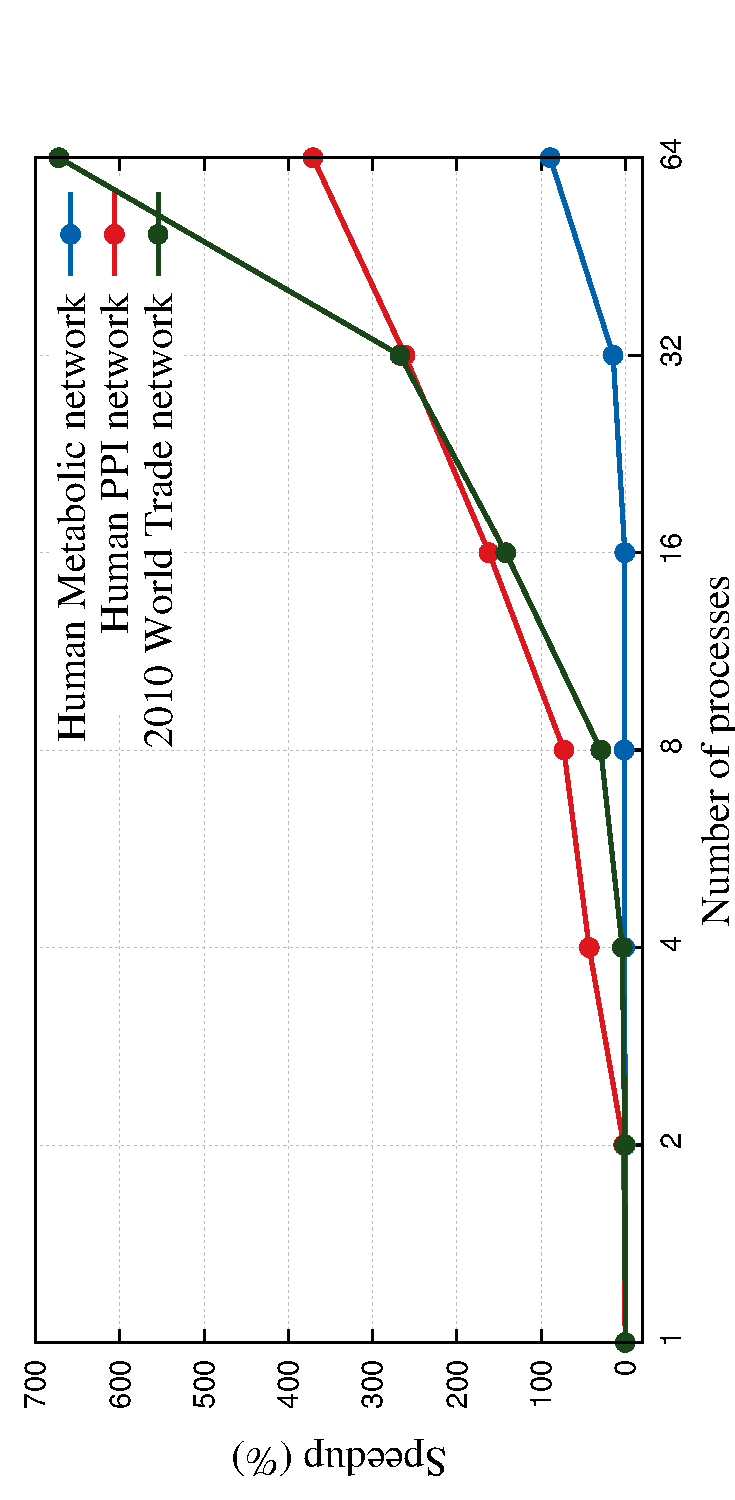
\includegraphics[angle=-90,scale=0.45]{../code/final_results/parallelisation_results/nr_processes2}
  \label{fig:time_threads}
\end{figure}
  
\end{frame}


\newcommand{\cellsizegcvtable}{1.45}

\rowcolors{1}{blue1}{blue2}

\newcommand{\gcvtable}{
\begin{tabular}{p{\cellsizegcvtable cm}p{\cellsizegcvtable cm}p{\cellsizegcvtable cm}p{\cellsizegcvtable cm}p{\cellsizegcvtable cm}p{0.5cm}}
 Graphlets    & GCV (node 1) & GCV (node 2) & GCV (node 3) & GCV (node 4) & \dots \\
 G1 & 2 & 3 & 6 & 9 & \dots \\ 
 G2 & 1 & 10 & 23 & 0 & \dots \\ 
 G3 & 0 & 3 & 5 & 14 & \dots \\ 
 G4 & 4 & 9 & 6 & 2 & \dots \\ 
 \dots &  \dots & \dots & \dots & \dots & \dots\\
 G29 & 1 & 14 & 6 & 0 & \dots \\  
\end{tabular}
}
% diagram of computation process
\begin{frame}
  \frametitle{Pearson's GCV correlation matrices - computation}
  
%%%%%%%%%% GCV computation process %%%%%%%%%%%%%



\begin{figure}[h]
  \begin{center}
  \begin{tikzpicture}[scale=0.55,auto,swap,post/.style={->,shorten >=3pt,>=stealth',thick}, every node/.style={scale=0.55}]


    \node[inner sep=0pt] (1a) at (-9.0, 2.0) {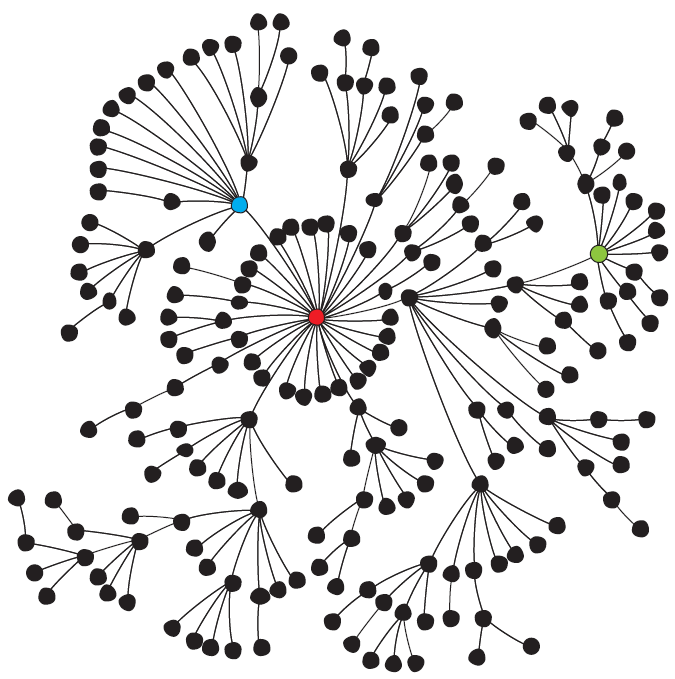
\includegraphics[width=0.4\textwidth]{../report_imperial/images/scale-free-network.png}};
    \node[inner sep=0pt] (2a) at (-6.5, 9.0) {\gcvtable};
    \node[inner sep=0pt] (3a) at (-0.0, 2.0) {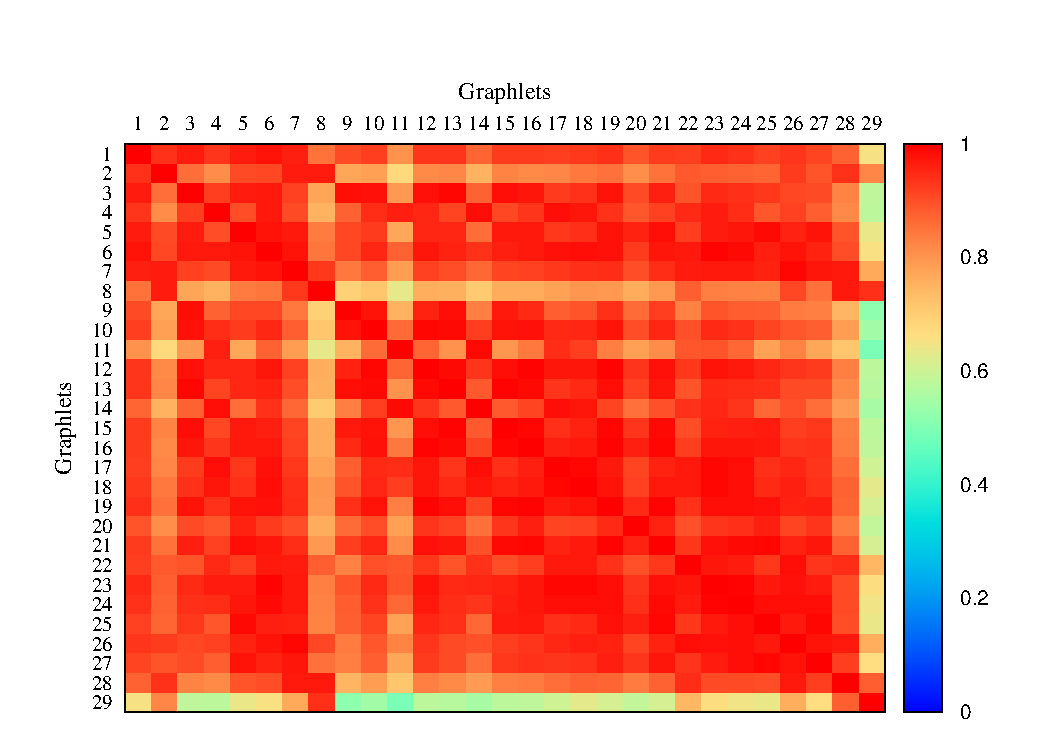
\includegraphics[scale=0.7]{../code/final_results/human_ppi/heatmap_pearsons_human_ppi2.pdf}};
    \node[text width=10em] (4a) at (2.5, 8.7) {$\rho(i,j) = $ Pearson's correlation between row vectors $i$ and $j$ };
    \node (5a) at (2.5, 1) {};
    \node (gcv_src) at (-1.0, 8.7) {};
    
    \draw[red] (-12.0,9.5) rectangle (-1.0,9.0);
    \draw[red] (-12.0,8.55) rectangle (-1.0,8.05);
	  
   \draw[post] (1a) -- node[right] {Graphlet Cluster Vectors (GCVs)} (1a |- 2a.south);
%     \path[hi, line width=1.0]  (4a)  -- (5a);
    \draw[post] (2.5, 8.0)-|(5a.north);
    \draw[post,rounded corners=5pt] (gcv_src) -- node[above] {} (gcv_src -| 4a.west) ;
    
  \end{tikzpicture}
%   \caption{}
  \label{fig:gcv_corr_process}
  \end{center}
\end{figure}%

%%%%%%%%%%%%%%%%%%%%%%%
  
\end{frame}

\rowcolors{1}{}{}
\newcommand{\heatmaptxtscaling}{1.5}

\def\myarm{1cm}
\def\myangle{0}
\tikzset{
  arm/.default=1cm,
  arm/.code={\def\myarm{#1}}, % store value in \myarm
  angle/.default=0,
  angle/.code={\def\myangle{#1}} % store value in \myangle
}

% Define the myncbar to path
\tikzset{
    myncbar/.style = {to path={
        % We need to calculate a couple of coordinates to help us draw
        % the path. 
        let
            % Same as (\tikztotarget)++(\myangle:\myarm)
            \p1=($(\tikztotarget)+(\myangle:\myarm)$)
        in
            -- ++(\myangle:\myarm) coordinate (tmp)
            % Find the projection of the (tmp) coordinate
            % on the line from the target to p1
            --  node[below,scale=\heatmaptxtscaling] {\hspace{1.0em}\begin{tabular}{c} $4^{th}$ degree polynomial scaling: \\ $x' = x^4$ \end{tabular}} ($(\tikztotarget)!(tmp)!(\p1)$)
            -- (\tikztotarget)\tikztonodes
    }}
}


% normalisation process
\begin{frame}
 \frametitle{Correlation Matrix Normalisation Process}
 
 %%%%%%%%%% Heatmap life cycle %%%%%%%%%%%%%

% Define the arm and angle options


\begin{figure}[h]
%   \rowcolors{1}{}{}
%   \hspace{-3.0em}
  \centering
  \begin{tikzpicture}[scale=0.47,auto,swap,post/.style={->,shorten >=3pt,>=stealth',thick}, every node/.style={scale=0.47}]

    \node[inner sep=0pt] (orig) at (0.0, 8.0) {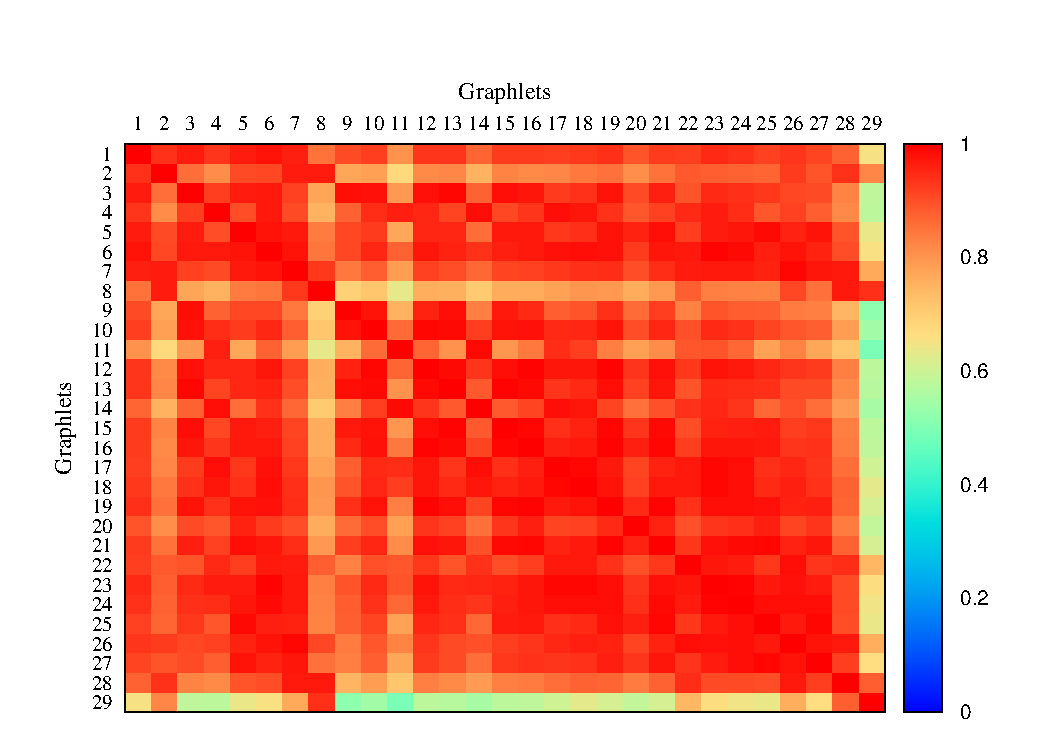
\includegraphics[scale=0.5]{../code/final_results/human_ppi/heatmap_pearsons_human_ppi2.pdf}};
    \node[scale=\heatmaptxtscaling] at (orig.north) {\textbf{Initial matrix}};
    \node[inner sep=0pt] (feature_scaled) at (0.0, 0.0) {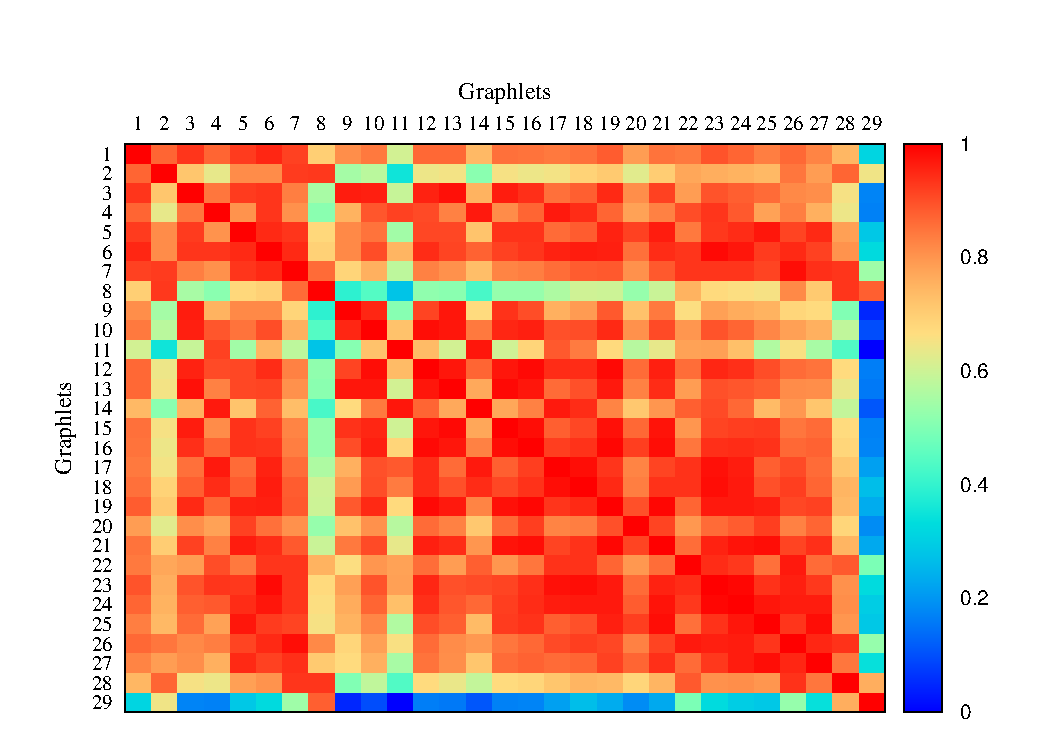
\includegraphics[scale=0.5]{../code/final_results/human_ppi/heatmap_pearsons_normalized_human_ppi2.pdf}};
    \node[inner sep=0pt] (poly4) at (9.0, 0.0) {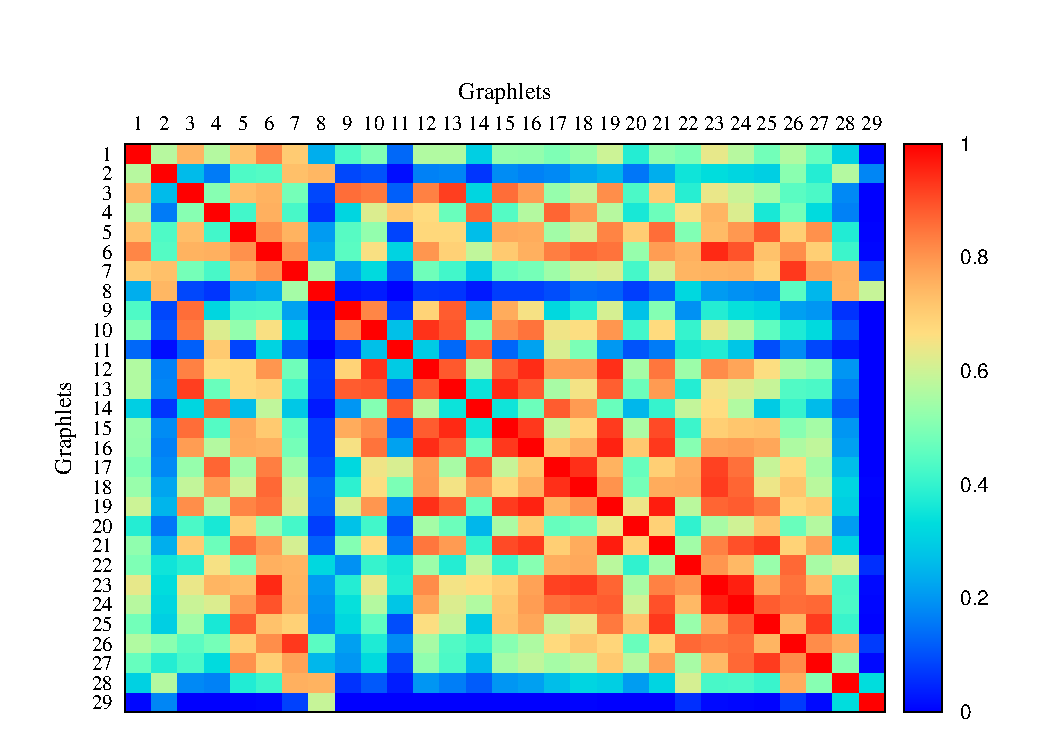
\includegraphics[scale=0.5]{../code/final_results/human_ppi/heatmap_pearsons_normalized_human_ppi-poly-42.pdf}};
    \node[inner sep=0pt] (hclust) at (9.0, 8.0) {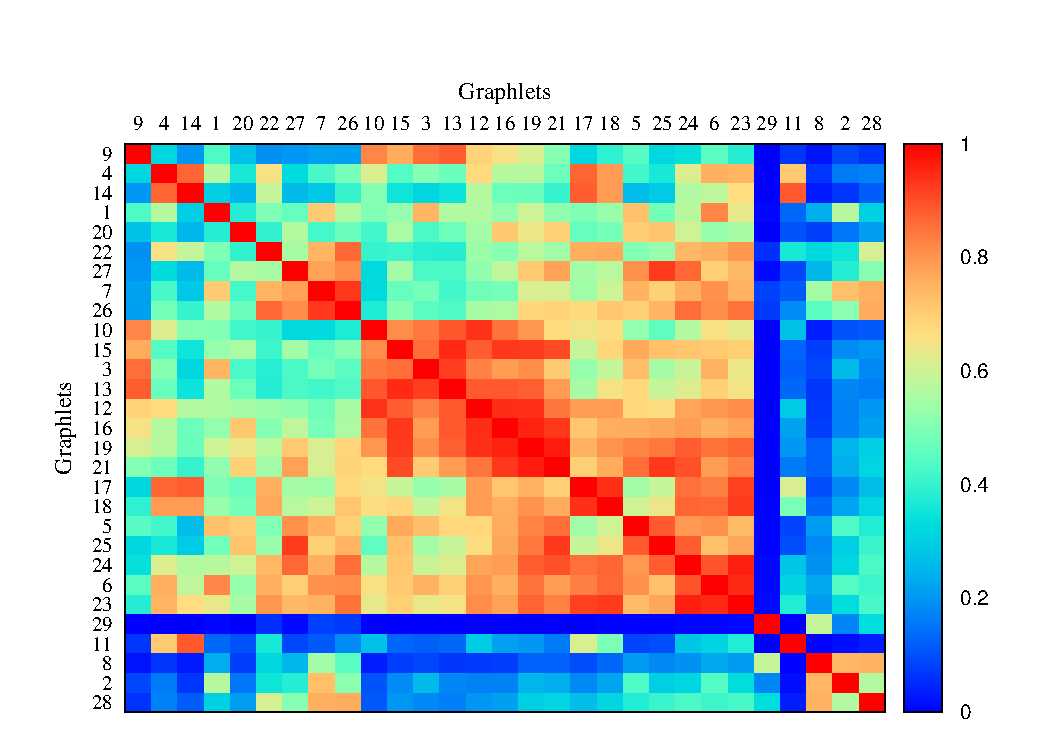
\includegraphics[scale=0.5]{../code/final_results/human_ppi/heatmap_pearsons_hclust_human_ppi-poly-42.pdf}};
    \node[scale=\heatmaptxtscaling] at (hclust.north) {\textbf{Final matrix}};
    
    \draw[line,thick, ->] (orig) -- node[right,scale=\heatmaptxtscaling] {\begin{tabular}{l} feature scaling: \\ $x' = \frac{x - min}{max - min}$ \end{tabular}} (feature_scaled) {};
    \draw [->,thick] (feature_scaled.south)  to[myncbar,arm=-0.5cm,angle=90]  (poly4.south);
    \draw[line,thick, ->] (poly4) -- node[right,scale=\heatmaptxtscaling] {\begin{tabular}{l}hierarchical clustering\\(complete linkage)\end{tabular}} (hclust) {};


  \end{tikzpicture}
%   \caption[Pearson's GCV correlation matrix life cycle for the Human PPI network]{Pearson's GCV correlation matrix life cycle for the Human PPI network. The initial Pearson's GCV correlation matrix is on the top-left corner and the final matrix is on the top-right corner, after feature scaling, polynomial scaling and hierarchical clustering operations are applied. One can see that in the final matrix graphlet clusters are distinguished more easily compared to the initial matrix. The operation order is anti-clockwise. When feature scaling, the range of the correlations $[min, max]$ is scaled to $[0,1]$. After performing polynomial scaling using a $4^{th}$ degree function, the correlations are lowered even more. Finally, after applying hierarchical clustering, similar graphlets cluster together along the diagonal. Hierarchical clustering uses complete linkage for grouping GCVs and the Euclidean distance to compute the difference between GCVs.}
  \label{fig:heatmap_process}
\end{figure}%

%%%%%%%%%%%%%%%%%%%%%%%
 
\end{frame}


\begin{frame}
 \frametitle{Presentation outline}
 
 \begin{itemize}
  \item GCV Implementation \vfill
  \item \textcolor{red}{Applications} \vfill
  
  \begin{figure}
    \hspace{-3em}
    \begin{tikzpicture}[scale=0.7,auto,swap]


    \node[inner sep=0pt] (trade) at (-5.5, 0.5) {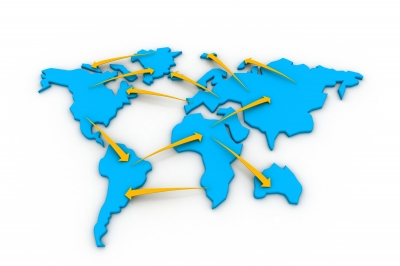
\includegraphics[width=0.33\textwidth]{images/world_trade_net.jpg}};
    \node[inner sep=0pt] (ppi) at (0, 0.0) {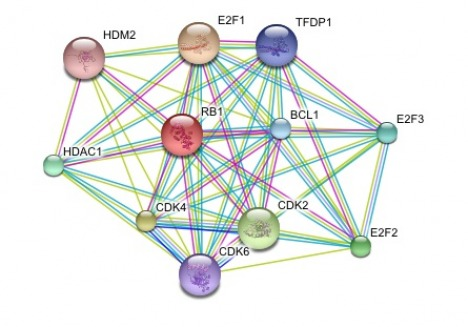
\includegraphics[width=0.33\textwidth]{images/protein_network.jpg}};
    \node[inner sep=0pt] (meta) at (5.5, 0.0) {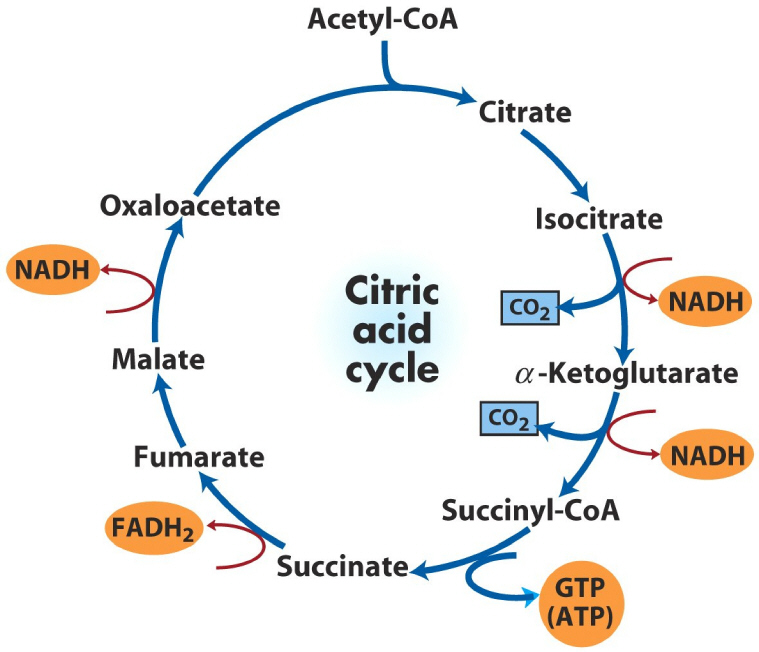
\includegraphics[scale=0.5]{images/metabolic_net.jpg}};

    \node[inner sep=0pt] (trade_label) at (-5.5,3) {\begin{tabular}{c} World Trade\\ networks \end{tabular}};
    \node[inner sep=0pt] (ppi_label) at (0,3) {\begin{tabular}{c} Protein Interaction\\ networks \end{tabular}};
    \node[inner sep=0pt] (meta_label) at (5.5,3) {\begin{tabular}{c} Metabolic\\ networks \end{tabular} };

    \end{tikzpicture}
  \end{figure}
  \item Evaluation on random graphs clustering \vfill
 \end{itemize}
 
\end{frame}




% give example of the Pearson's GCV matrix
\begin{frame}
  \frametitle{Pearson's GCV correlation matrix - World Trade network}
  
%   \begin{figure}
%    \vspace{-0.5in}
%    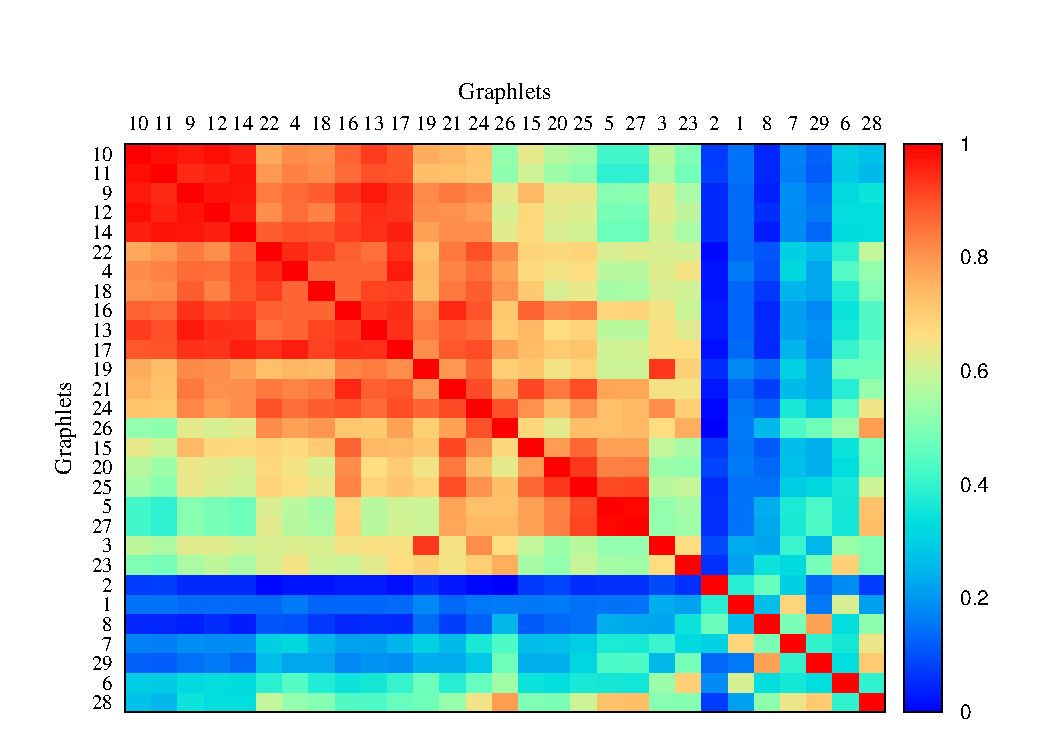
\includegraphics[scale=0.6]{../code/final_results_norm1/trade_2010_thresholded/heatmap_pearsons_hclust_trade_2010_thresholded2.pdf}
%   \end{figure}


  \begin{figure}
   \vspace{-0.2in}
    \begin{tikzpicture}[scale=0.7,auto,swap]


    \node[inner sep=0pt] (trade) at (0, 0.15) {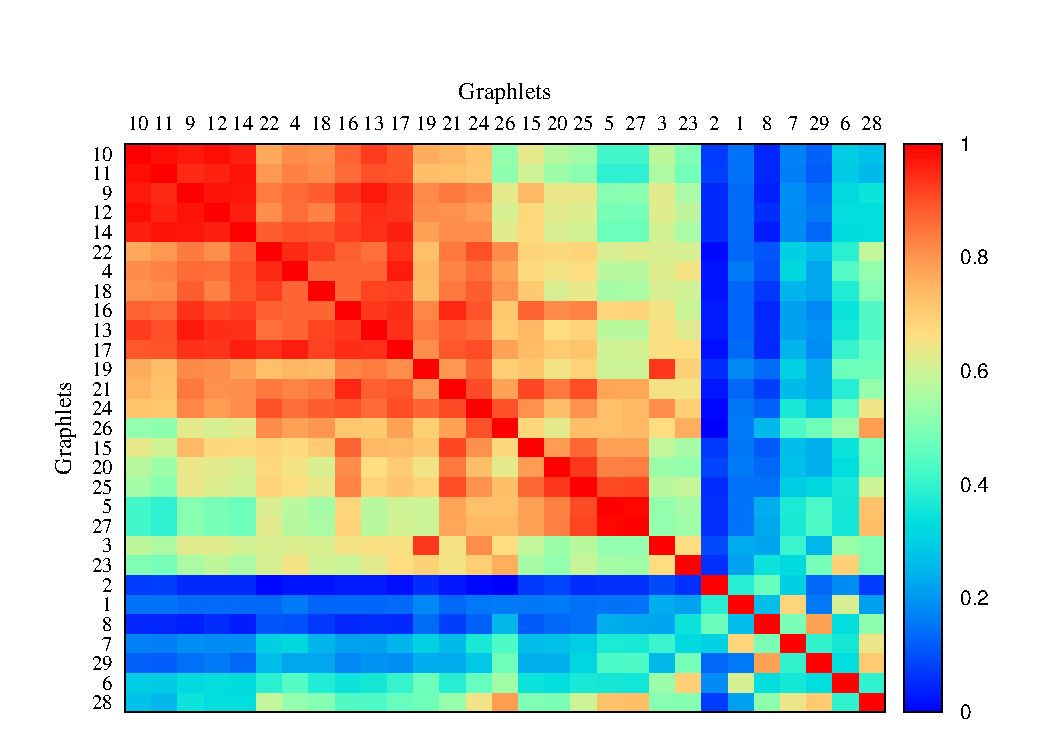
\includegraphics[scale=0.55]{../code/final_results_norm1/trade_2010_thresholded/heatmap_pearsons_hclust_trade_2010_thresholded2.pdf}};
    \node[inner sep=0pt,scale=0.5] (g10) at (-8.5, 3) {\gtenpic};
    \node[inner sep=0pt,scale=0.5] (g10_lab) at (-9.3, 3) {\LARGE{$G_{10}$}};

    \node[inner sep=0pt,scale=0.5] (g11) at (-8.5, 1) {\gelevenpic};
    \node[inner sep=0pt,scale=0.5] (g11_lab) at (-9.6, 1) {\LARGE{$G_{11}$}};

    \node[inner sep=0pt,scale=0.5] (g9) at (-8.5, -1.5) {\gninepic};
    \node[inner sep=0pt,scale=0.5] (g9_lab) at (-9.3, -1.5) {\LARGE{$G_{9}$}};

    \node[inner sep=0pt,scale=0.5] (g12) at (-8.5, -4) {\gtwelvepic};
    \node[inner sep=0pt,scale=0.5] (g12_lab) at (-9.5, -4) {\LARGE{$G_{12}$}};

    \node[inner sep=0pt,scale=0.5] (g2) at (-6, -6.5) {\gtwopic};
    \node[inner sep=0pt,scale=0.5] (g2_lab) at (-6.8, -6.5) {\LARGE{$G_{2}$}}; 

    \node[inner sep=0pt,scale=0.5] (g8) at (-2.66, -6.5) {\geightpic};
    \node[inner sep=0pt,scale=0.5] (g8_lab) at (-3.5, -6.5) {\LARGE{$G_{8}$}};

    \node[inner sep=0pt,scale=0.5] (g7) at (0.66, -6.5) {\gsevenpic};
    \node[inner sep=0pt,scale=0.5] (g7_lab) at (-0.5, -6.5) {\LARGE{$G_{7}$}};
    
    \node[inner sep=0pt,scale=0.5] (g29) at (4.0, -6.5) {\gtwentyninepic};
    \node[inner sep=0pt,scale=0.5] (g29_lab) at (2.8, -6.5) {\LARGE{$G_{29}$}};
    
    \draw[line] (g10) -| (-7,3) -- (-6, 3);
    \draw[line] (-7.6, 1) -| (-7.2,2.75) -- (-6, 2.75);
    \draw[line] (-8.1, -1.5) -| (-7,2.45) -- (-6, 2.45);
    \draw[line] (-7.7, -4) -| (-6.8,2.2) -- (-6, 2.2);
    
    \draw[line] (-6, -5.6) |- (2.5,-4.9) -- (2.5, -4.7);
    \draw[line] (-2.66, -5.6) |- (3.2,-5.1) -- (3.2, -4.7);
    \draw[line] (0.66, -5.6) |- (3.55,-5.3) -- (3.55, -4.7);
    \draw[line] (4.0, -5.6) |- (3.9,-5.1) -- (3.9, -4.7);
    
    
   \end{tikzpicture}

  \end{figure}

\end{frame}



\begin{frame}
  \frametitle{Correlation matrix change during 1962--2010}
  
  \begin{figure}
   \vspace{-0.25in}
   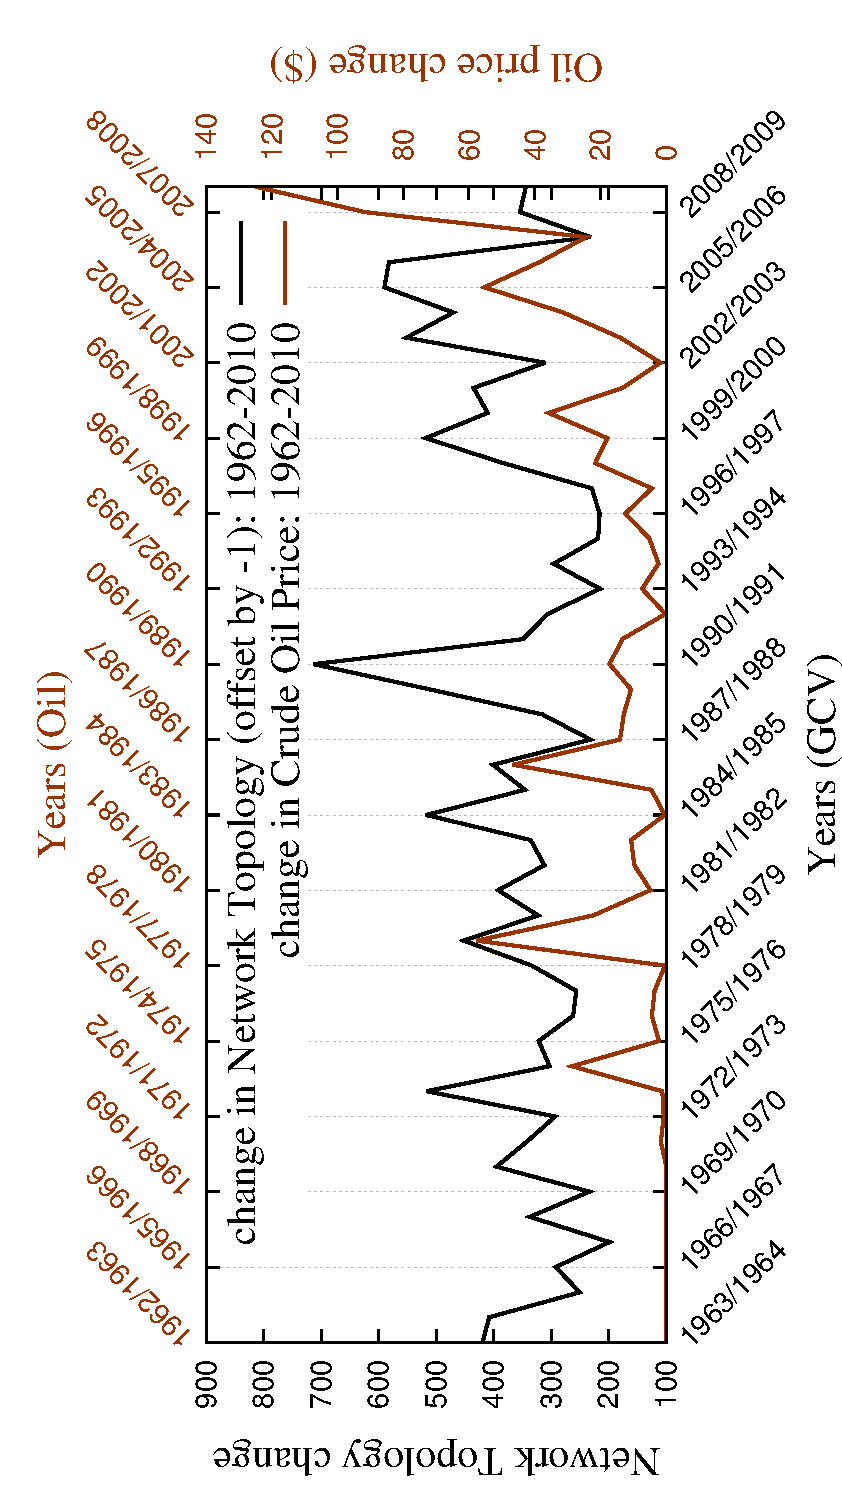
\includegraphics[angle=-90,scale=0.45]{../code/final_results_norm1/all_trade_thresh/change_over_time2}
  \end{figure}

  \begin{itemize}
   \item Spearman's correlation: 0.34
   \item p-value: 0.01
   \item offset: -1 $\implies$ \textcolor{red}{the network topology causes the changes in oil price!}
  \end{itemize}

  
\end{frame}

\newcommand{\ccaIndicatorsTradeNorm}{
  \begin{tabular}{r}
  \cellcolor{black}\textcolor{ccacol1}{POP}\\
  \cellcolor{black}\textcolor{ccacol1}{LE}\\
  \cellcolor{black}\textcolor{ccacol2}{KI}\\
  \cellcolor{black}\textcolor{ccacol2}{RGDPCH x POP}\\
  \cellcolor{black}\textcolor{ccacol2}{RGDPL x POP}\\
  \cellcolor{black}\textcolor{ccacol2}{RGDPL2 x POP}\\
  \cellcolor{black}\textcolor{ccacol2}{KG x RGDPL x POP}\\
  \cellcolor{black}\textcolor{ccacol2}{KC x RGDPL x POP}\\
  \cellcolor{black}\textcolor{ccacol3}{KC x RGDPL}\\
  \cellcolor{black}\textcolor{ccacol4}{XRAT}\\
  \cellcolor{black}\textcolor{ccacol4}{RGDPCH}\\
  \cellcolor{black}\textcolor{ccacol4}{RGDPL}\\
  \cellcolor{black}\textcolor{ccacol4}{RGDPL2}\\
  \cellcolor{black}\textcolor{ccacol4}{KG x RGDPL}\\
  \cellcolor{black}\textcolor{ccacol4}{KI x RGDPL}\\
  \cellcolor{black}\textcolor{ccacol4}{KC}\\
  \cellcolor{black}\textcolor{ccacol5}{KI}\\
  \cellcolor{black}\textcolor{ccacol5}{BCA per RGDPL}\\
  \cellcolor{black}\textcolor{ccacol5}{KG}\\
  \cellcolor{black}\textcolor{ccacol5}{BCA}\\
  \cellcolor{black}\textcolor{ccacol6}{OPENK}
  \end{tabular}

}


% CCA - on the Trade network - 
\begin{frame}
  \frametitle{Canonical Correlation Analysis (CCA)}

\begin{figure}[H]
  \centering
    \begin{tikzpicture}[scale=\ccafigscale,show background rectangle, 
  background rectangle/.style={fill=black},
  color=white,help lines/.style={color=lightgray,line width=0.2pt},post/.style={->,shorten >=1pt,>=stealth',thick}]

    \node[upper left,inner sep=0,scale=\ccafigscale] (indicators) at (-2.0,0) {\ccaIndicatorsTradeNorm};	
    \shade[top color=green,bottom color=yellow] (4,0) rectangle (4.5,5);
    \shade[top color=yellow,bottom color=red] (4,-5) rectangle (4.5,0);
    \node[upper left,inner sep=0] (dummy) at (13.0,4) {}; % for extending the black bounding box
    \node[upper left,inner sep=0] (corr_text) at (4.25,-6.5) {Correlation};
    \node[upper left,inner sep=0,red] (corr_text) at (4.25,-5.5) {-1};
    \node[upper left,inner sep=0, green] (corr_text) at (4.25,5.5) {1};
    \node[upper left,inner sep=0] (corr_text) at (4.75,0) {0};
    
    \node[upper left,inner sep=0,scale=\ccafigscale] (g12) at (7.5,4.0) {\gtwelvecca{ccacol1}};
    \node[upper left,inner sep=0,scale=\ccafigscale] (g10) at (10.5,2.5) {\gtencca{ccacol1}};
    \node[upper left,inner sep=0,scale=\ccafigscale] (g14) at (7.5,1.0) {\gfourteencca{ccacol1}};
    \node[upper left,inner sep=0,scale=\ccafigscale] (g2) at (10.5,-1.0) {\gtwocca{ccacol8}};
    \node[upper left,inner sep=0,scale=\ccafigscale] (g29) at (7.5,-2.5) {\gtwentyninecca{ccacol8}};
    \node[upper left,inner sep=0,scale=\ccafigscale] (g8) at (10.5,-4.0) {\geightcca{ccacol8}};
    
    
%     \draw[line,color=ccacol1] (0,4.8) -| (3,5) -- (4.25,5); % top-left elem
%     \draw[line,color=ccacol1] (0,4.35) -| (2,3.9) -- (4.25,3.9); % next in line
    
    \draw[line,color=ccacol1] (0.00,4.80) -| (1.75,3.68) -- (4.00,3.68);
    \draw[line,color=ccacol1] (0.00,4.33) -| (1.49,3.58) -- (4.00,3.58);
    \draw[line,color=ccacol1] (0.00,3.85) -| (1.37,3.30) -- (4.00,3.30);
    \draw[line,color=ccacol1] (0.00,3.38) -| (1.07,3.27) -- (4.00,3.27);
    \draw[line,color=ccacol1] (0.00,2.90) -| (1.25,3.27) -- (4.00,3.27);
    \draw[line,color=ccacol1] (0.00,2.42) -| (1.56,3.26) -- (4.00,3.26);
    \draw[line,color=ccacol1] (0.00,1.95) -| (1.84,3.21) -- (4.00,3.21);
    \draw[line,color=ccacol1] (0.00,1.48) -| (2.13,3.17) -- (4.00,3.17);
    \draw[line,color=ccacol3] (0.00,1.00) -| (1.31,1.46) -- (4.00,1.46);
    \draw[line,color=ccacol4] (0.00,0.53) -| (1.22,0.85) -- (4.00,0.85);
    \draw[line,color=ccacol4] (0.00,0.05) -| (1.50,0.80) -- (4.00,0.80);
    \draw[line,color=ccacol4] (0.00,-0.42) -| (1.82,0.80) -- (4.00,0.80);
    \draw[line,color=ccacol4] (0.00,-0.90) -| (2.13,0.80) -- (4.00,0.80);
    \draw[line,color=ccacol4] (0.00,-1.38) -| (2.30,0.79) -- (4.00,0.79);
    \draw[line,color=ccacol4] (0.00,-1.85) -| (2.58,0.52) -- (4.00,0.52);
    \draw[line,color=ccacol4] (0.00,-2.33) -| (2.68,0.43) -- (4.00,0.43);
    \draw[line,color=ccacol5] (0.00,-2.80) -| (2.77,-0.08) -- (4.00,-0.08);
    \draw[line,color=ccacol5] (0.00,-3.27) -| (2.92,-0.55) -- (4.00,-0.55);
    \draw[line,color=ccacol5] (0.00,-3.75) -| (3.07,-0.64) -- (4.00,-0.64);
    \draw[line,color=ccacol5] (0.00,-4.23) -| (3.32,-0.75) -- (4.00,-0.75);
    \draw[line,color=ccacol6] (0.00,-4.70) -| (3.55,-1.33) -- (4.00,-1.33);

    \draw[line,color=ccacol1] (g12) -| (5.5,4.5) -- (4.5,4.5);
    \draw[line,color=ccacol1] (g10) -| (5.3,4.47) -- (4.5,4.47);
    \draw[line,color=ccacol1] (g14) -| (5.1,4.43) -- (4.5,4.43);

    \draw[line,color=ccacol8] (g2) -| (5.3,-2.5) -- (4.5,-2.5);
    \draw[line,color=ccacol8] (g29) -| (5.5,-3) -- (4.5,-3);
    \draw[line,color=ccacol8] (g8) -| (5.1,-3.5) -- (4.5,-3.5);
    
    \end{tikzpicture}
    \label{fig:all_trade_cca_black}	
\end{figure}
\end{frame}


\begin{frame}
  \frametitle{Trading partners sparsity index}
  \begin{itemize}
   \item Measures how sparse the neighbourhood of a node is. \vfill
   \item $ T =  \underbrace{
   \textcolor{darkgreen2}{w_{12}}F_{12} + 
   \textcolor{darkgreen2}{w_{10}}F_{10} + 
   \textcolor{darkgreen2}{w_{14}}F_{14}}_{\textcolor{darkgreen2}{\text{sparse graphlets}}} + \underbrace{
   \textcolor{red}{w_{8}}F_{8} + 
   \textcolor{red}{w_{29}}F_{29} + 
   \textcolor{red}{w_{2}}F_{2}}_{\textcolor{red}{\text{dense graphlets}}}$ \vfill
   \item can have both positive or negative values \vfill
  \end{itemize}

\end{frame}

% USA, China, Ger, etc ..
\begin{frame}
  \frametitle{Trading partners sparsity index -- G20}
  
  \begin{figure}
    \centering
    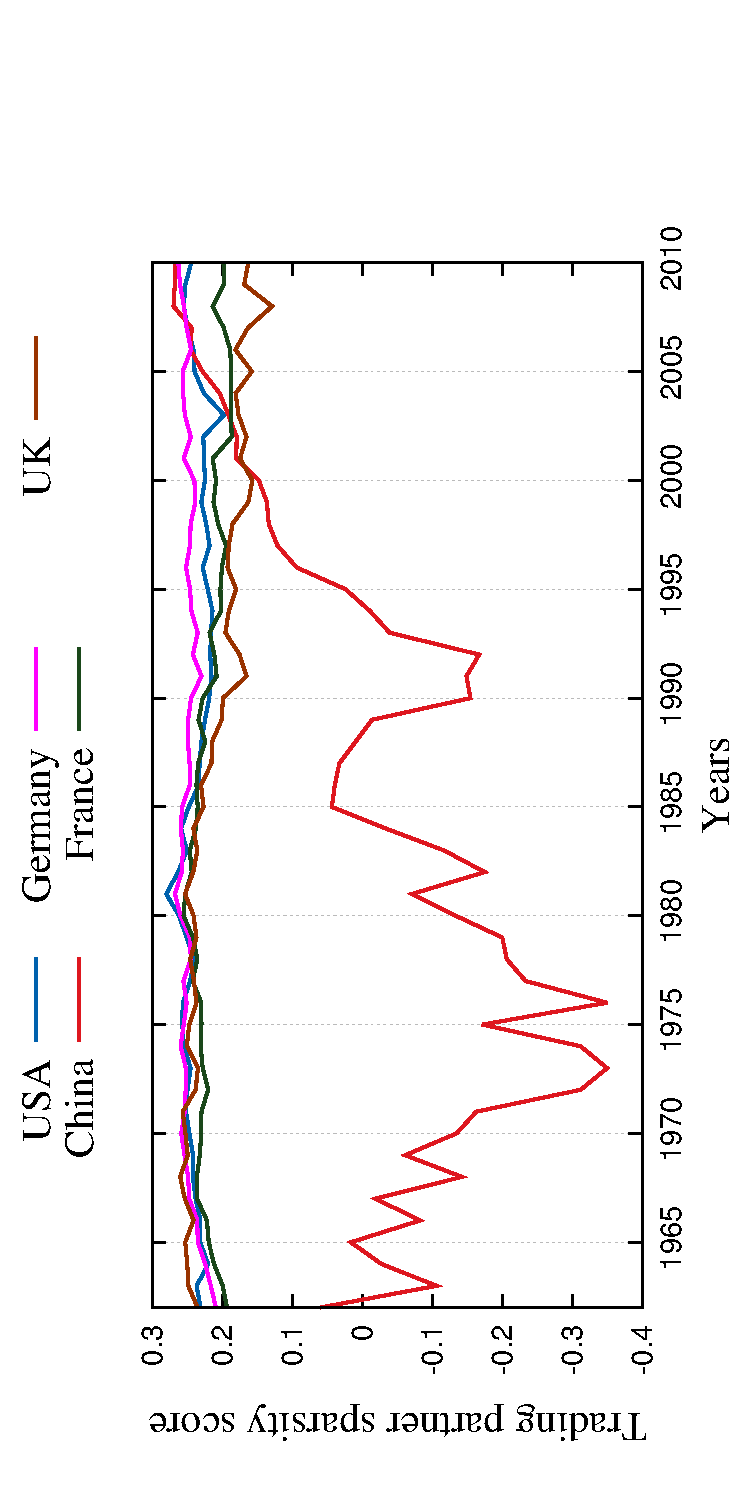
\includegraphics[angle=-90,scale=0.5]{../code/extra_results/trading_partner_density/scores/g722.pdf}
  \end{figure}

\end{frame}


\begin{frame}
  \frametitle{Trading partners sparsity index -- Eastern Europe}

  \begin{figure}
    \centering
    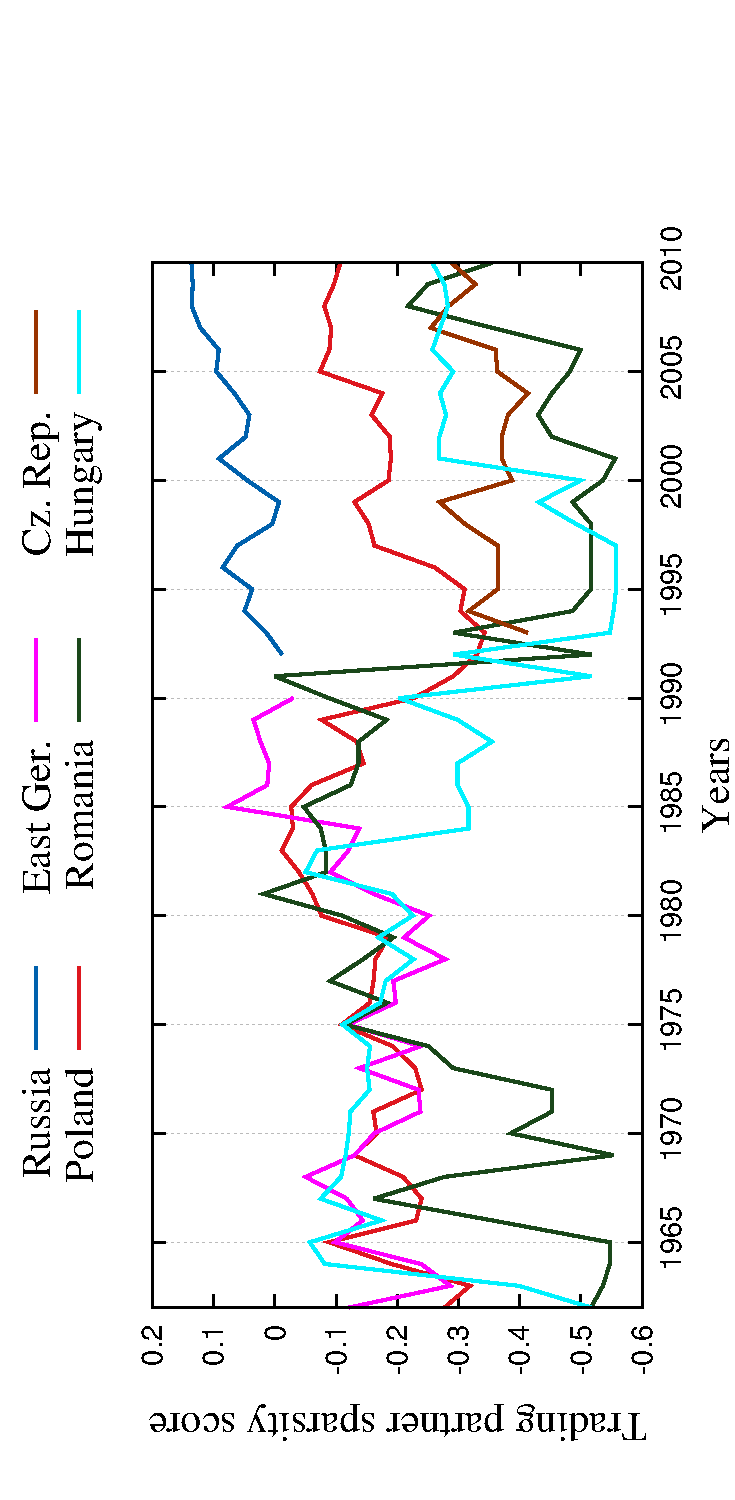
\includegraphics[angle=-90,scale=0.5]{../code/extra_results/trading_partner_density/scores/eastern_europe22.pdf}
  \end{figure}
\end{frame}


\begin{frame}
  \frametitle{Trading partners sparsity index -- OPEC}
    \begin{figure}
    \centering
    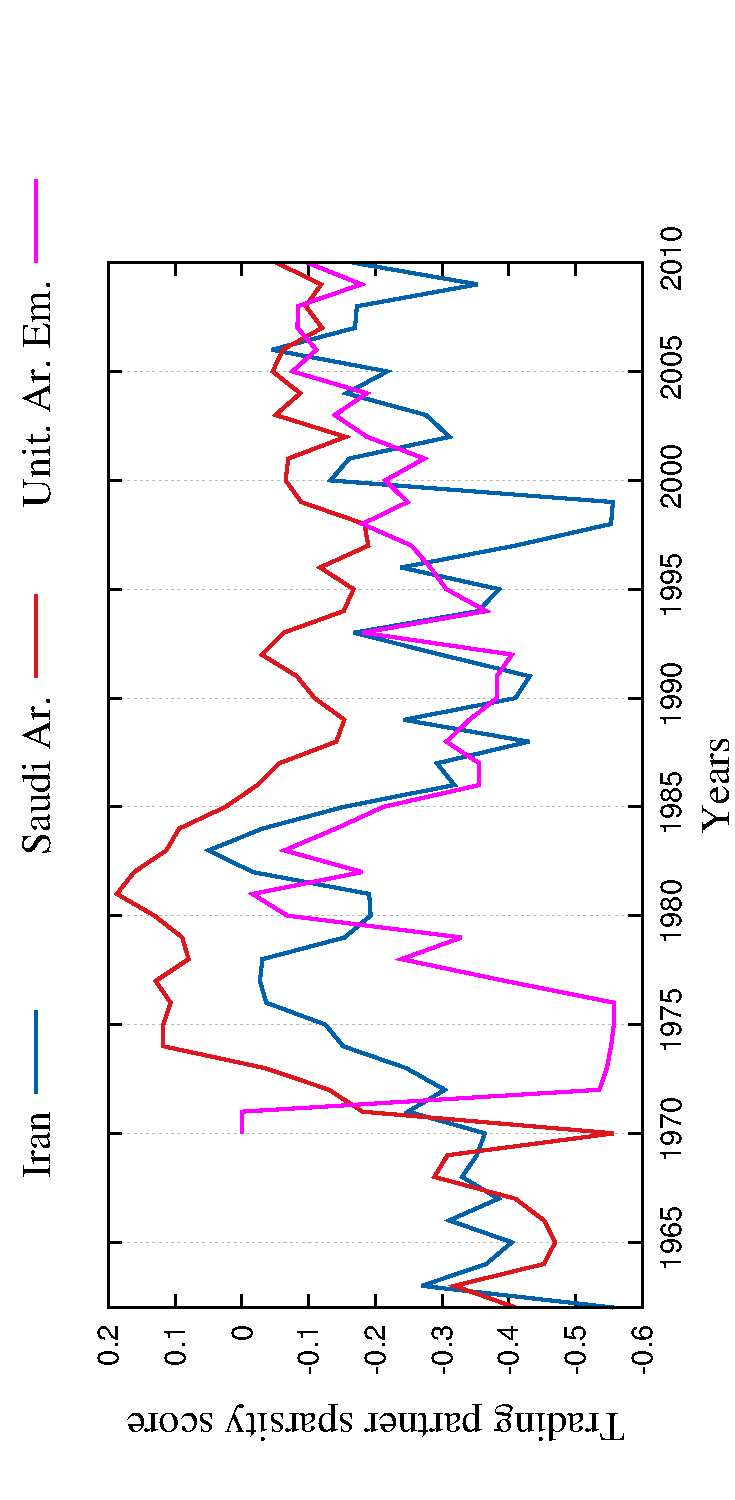
\includegraphics[angle=-90,scale=0.5]{../code/extra_results/trading_partner_density/scores/opec22.pdf}
  \end{figure}
\end{frame}


\newcommand{\ccaIndicatorsRTA}{
\LARGE{
  \begin{tabular}{r}
  \cellcolor{black}\textcolor{ccacol1}{Goods RTAs}\\
  \\
  \cellcolor{black}\textcolor{ccacol1}{Physical RTAs}\\
  \\
  \cellcolor{black}\textcolor{ccacol4}{Services EIAs}
  \end{tabular}
}
}


% CCA - on RTAs
% \begin{frame}
%   \frametitle{CCA -- Integration using Regional Trade Agreements}
% 
% \begin{figure}[H]
%   \centering
%     \begin{tikzpicture}[scale=\ccafigscale,show background rectangle, 
%   background rectangle/.style={fill=black},
%   color=white,help lines/.style={color=lightgray,line width=0.2pt},post/.style={->,shorten >=1pt,>=stealth',thick}]
% 
%     \node[upper left,inner sep=0,scale=\ccafigscale] (indicators) at (-2.0,0) {\ccaIndicatorsRTA};	
%     \shade[top color=green,bottom color=yellow] (4,0) rectangle (4.5,5);
%     \shade[top color=yellow,bottom color=red] (4,-5) rectangle (4.5,0);
%     \node[upper left,inner sep=0] (dummy) at (13.0,4) {}; % for extending the black bounding box
%     \node[upper left,inner sep=0] (corr_text) at (4.25,-6.5) {Correlation};
%     \node[upper left,inner sep=0,red] (corr_text) at (4.25,-5.5) {-1};
%     \node[upper left,inner sep=0, green] (corr_text) at (4.25,5.5) {1};
%     \node[upper left,inner sep=0] (corr_text) at (4.75,0) {0};
%     
%     \node[upper left,inner sep=0,scale=\ccafigscale] (g2) at (7.5,4.0) {\gtwocca{ccacol1}};
%     \node[upper left,inner sep=0,scale=\ccafigscale] (g8) at (10.5,2.5) {\geightcca{ccacol1}};
%     \node[upper left,inner sep=0,scale=\ccafigscale] (g29) at (7.5,1.0) {\gtwentyninecca{ccacol1}};
%     \node[upper left,inner sep=0,scale=\ccafigscale] (g9) at (10.5,-1.0) {\gninecca{ccacol6}};
%     \node[upper left,inner sep=0,scale=\ccafigscale] (g11) at (7.5,-3.5) {\gelevencca{ccacol6}};
%     \node[upper left,inner sep=0,scale=\ccafigscale] (g10) at (10.5,-5.0) {\gtencca{ccacol6}};
%     
%     \draw[line,color=ccacol1] (0.00,1.5) -| (1.75,4.7) -- (4.00,4.7);
%     \draw[line,color=ccacol1] (0.00,0.0) -| (2.49,4.65) -- (4.00,4.65);
%     \draw[line,color=ccacol4] (0.00,-1.5) -| (3.37,0.2) -- (4.00,0.2);
%     
%     \draw[line,color=ccacol1] (g2) -| (5.1,4) -- (4.5,4);
%     \draw[line,color=ccacol1] (g8) -| (5.3,3.95) -- (4.5,3.95);
%     \draw[line,color=ccacol1] (g29) -| (5.1,3.9) -- (4.5,3.9);
% 
%     \draw[line,color=ccacol6] (g9) -| (5.3,-1.33) -- (4.5,-1.33);
%     \draw[line,color=ccacol6] (g11) -| (5.5,-1.40) -- (4.5,-1.4);
%     \draw[line,color=ccacol6] (g10) -| (5.1,-1.50) -- (4.5,-1.5);
%     
%     \end{tikzpicture}
%     \label{fig:all_trade_cca_black}	
% \end{figure}
% \end{frame}


\begin{frame}
  \frametitle{Case study -- Saudi Arabia}
  
  \begin{figure}
   \vspace{-0.25in}
   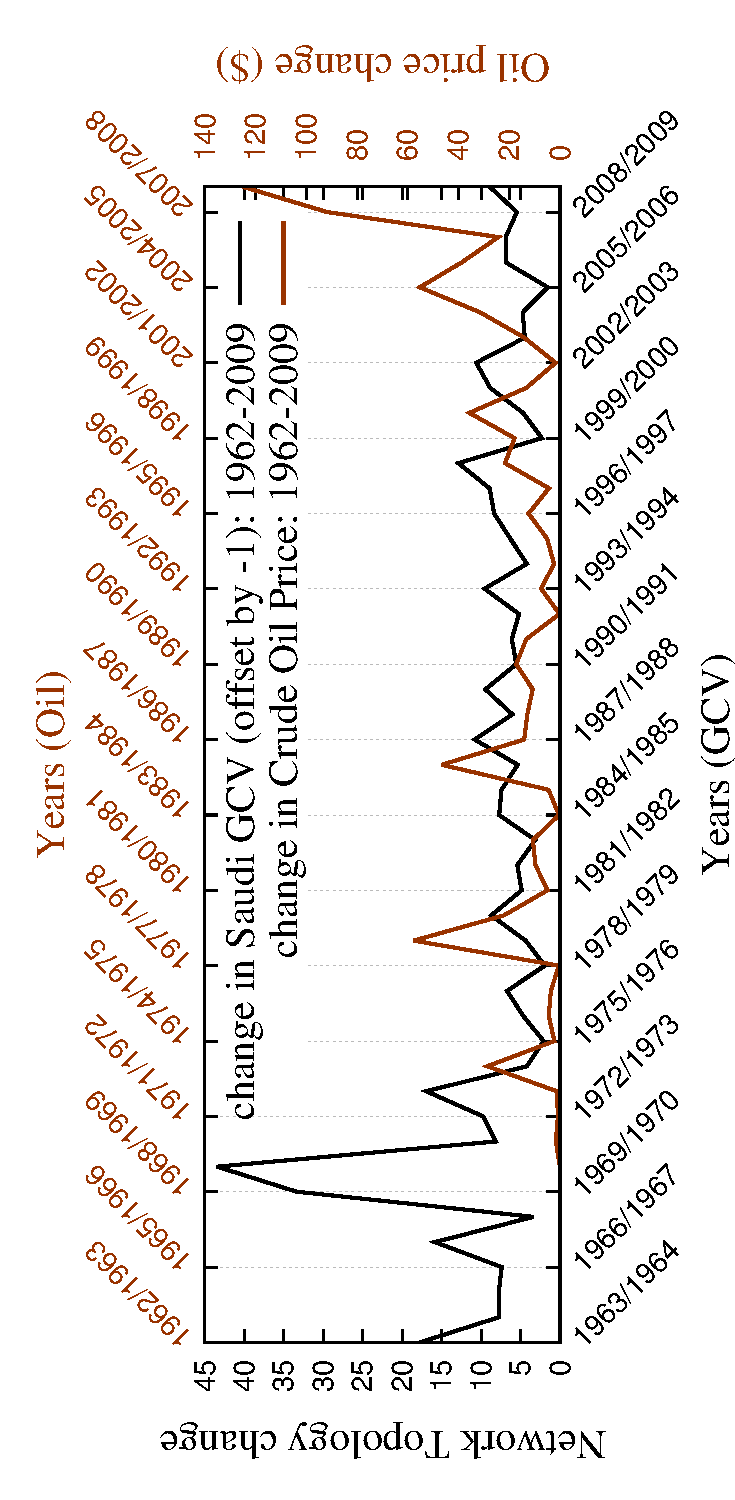
\includegraphics[angle=-90,scale=0.45]{../code/extra_results/saudi_oil/saudi_norm1_gcv_oil2}
  \end{figure}

  \begin{itemize}
   \item Spearman's correlation: -0.32
   \item p-value: 0.026
   \item offset: -1
  \end{itemize}

  
\end{frame}


% \rowcolors{1}{blue1}{blue2}
% \begin{frame}
%   \frametitle{Case study -- Saudi Arabia}
%   
%   \begin{figure}
%     
%     \centering
% 
%     \begin{tabular}{ c c | c c }
%     \multicolumn{2}{c}{Canonical Correlation} &  \multicolumn{2}{c}{0.82353} \\
%     \multicolumn{2}{c}{p-value} &  \multicolumn{2}{c}{0.00000} \\
%     \hline
%     \multicolumn{2}{c}{X variate} & \multicolumn{2}{c}{Y variate}\\
%     \hline
%     G3 & 0.49265 &  Crude Oil price & 0.83032\\
%     G6 & 0.09838 &  & \\
%     G4 & 0.05294 &  & \\
%     G5 & 0.03942 &  & \\
%     G7 & -0.23884 &  & \\
%     G8 & -0.46603 &  & \\
%     G2 & -0.50725 &  & \\
%     G1 & -0.52241 &  & \\
%     \end{tabular}
% 
%   \end{figure}
%   
%   \hilight{add black CCA image}
%   
% \end{frame}

% Mention that the metabolic will not be presented here, just mention the diseases, systems, bla bla
\begin{frame}
  \frametitle{Results for other networks}
  
  \begin{itemize}
    \item PPI networks -- key protein functions: \vfill
    \begin{itemize}
      \item Ribosome translation \vfill
      \item RNA processing \vfill
      \item Metabolism \vfill
      \item Golgi endosome vacuole sorting \vfill
    \end{itemize}
    \item Metabolic networks -- main results in: \vfill
    \begin{itemize}
      \item Cellular Processes \vfill
      \item Organismal Systems \vfill
      \item Human diseases \vfill
    \end{itemize}
 \end{itemize}
  
% \hilight{Add pictures for each of these}
  
\end{frame}


\rowcolors{1}{}{}
\begin{frame}
 \frametitle{Presentation outline}
 
 \begin{itemize}
  \item GCV Implementation \vfill
  \item Applications \vfill
  
  \begin{figure}
    \hspace{-3em}
    \begin{tikzpicture}[scale=0.7,auto,swap]


    \node[inner sep=0pt] (trade) at (-5.5, 0.5) {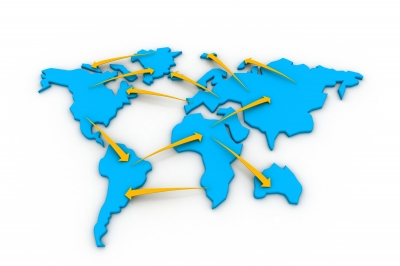
\includegraphics[width=0.33\textwidth]{images/world_trade_net.jpg}};
    \node[inner sep=0pt] (ppi) at (0, 0.0) {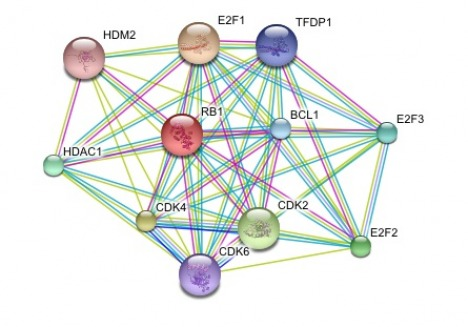
\includegraphics[width=0.33\textwidth]{images/protein_network.jpg}};
    \node[inner sep=0pt] (meta) at (5.5, 0.0) {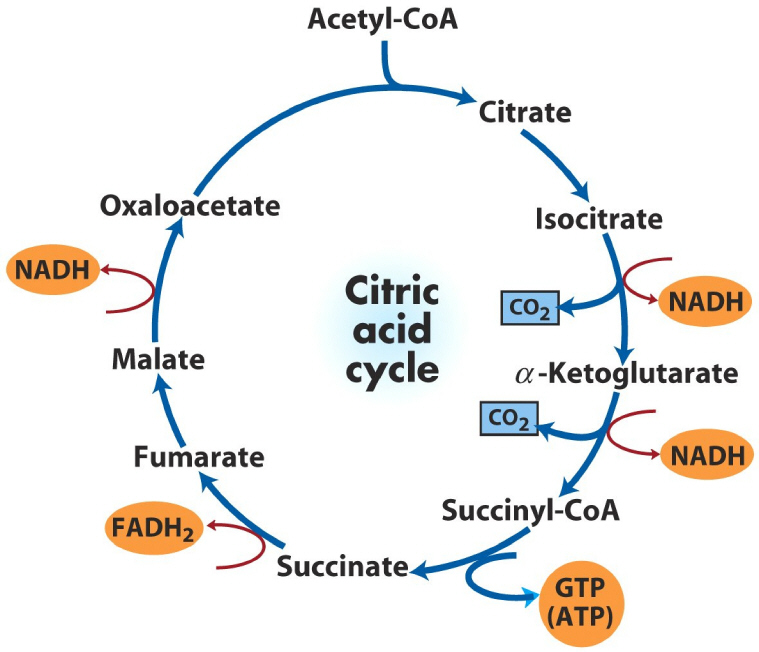
\includegraphics[scale=0.5]{images/metabolic_net.jpg}};

    \node[inner sep=0pt] (trade_label) at (-5.5,3) {\begin{tabular}{c} World Trade\\ networks \end{tabular}};
    \node[inner sep=0pt] (ppi_label) at (0,3) {\begin{tabular}{c} Protein Interaction\\ networks \end{tabular}};
    \node[inner sep=0pt] (meta_label) at (5.5,3) {\begin{tabular}{c} Metabolic\\ networks \end{tabular} };

    \end{tikzpicture}
  \end{figure}
  \item \textcolor{red}{Evaluation on random graphs clustering} \vfill
 \end{itemize}
 
\end{frame}



\begin{frame}
 \frametitle{Evaluation on random graphs clustering}
 We evaluated the GCV signature at classifying 5 random graphs: \vfill
\begin{itemize}
  \item Erd\H{o}s-R\'{e}nyi (ER) \vfill
  \item Erd\H{o}s-R\'{e}nyi (with preserved degree distribution) (ER-DD) \vfill 
  \item Geometric networks (GEO) \vfill
  \item Scale-free Barab\'{a}si-Albert -- preferential attachment (SF) \vfill
  \item Stickiness index-based (STICKY) \vfill
\end{itemize}


\end{frame}

\begin{frame}
 \frametitle{Other signatures evaluated}
 We compared the performance of GCV against 5 other signatures: \vfill
 \begin{itemize}
 \item Degree Distribution \vfill
 \item Average clustering coefficient \vfill
 \item Spectral distribution \vfill
 \item Graphlet Frequency Vector (GFV) -- RGFD distance \vfill
 \item Graphlet Distribution Vector (GDV) -- GCD73 distance \vfill
\end{itemize}

\end{frame}

\begin{frame}
  \frametitle{Multi-dimensional scaling}
  
  \begin{figure}[H] 
  \captionsetup{width=8cm}
  \centering
  \begin{minipage}[b]{0.50\linewidth}
    \centering
    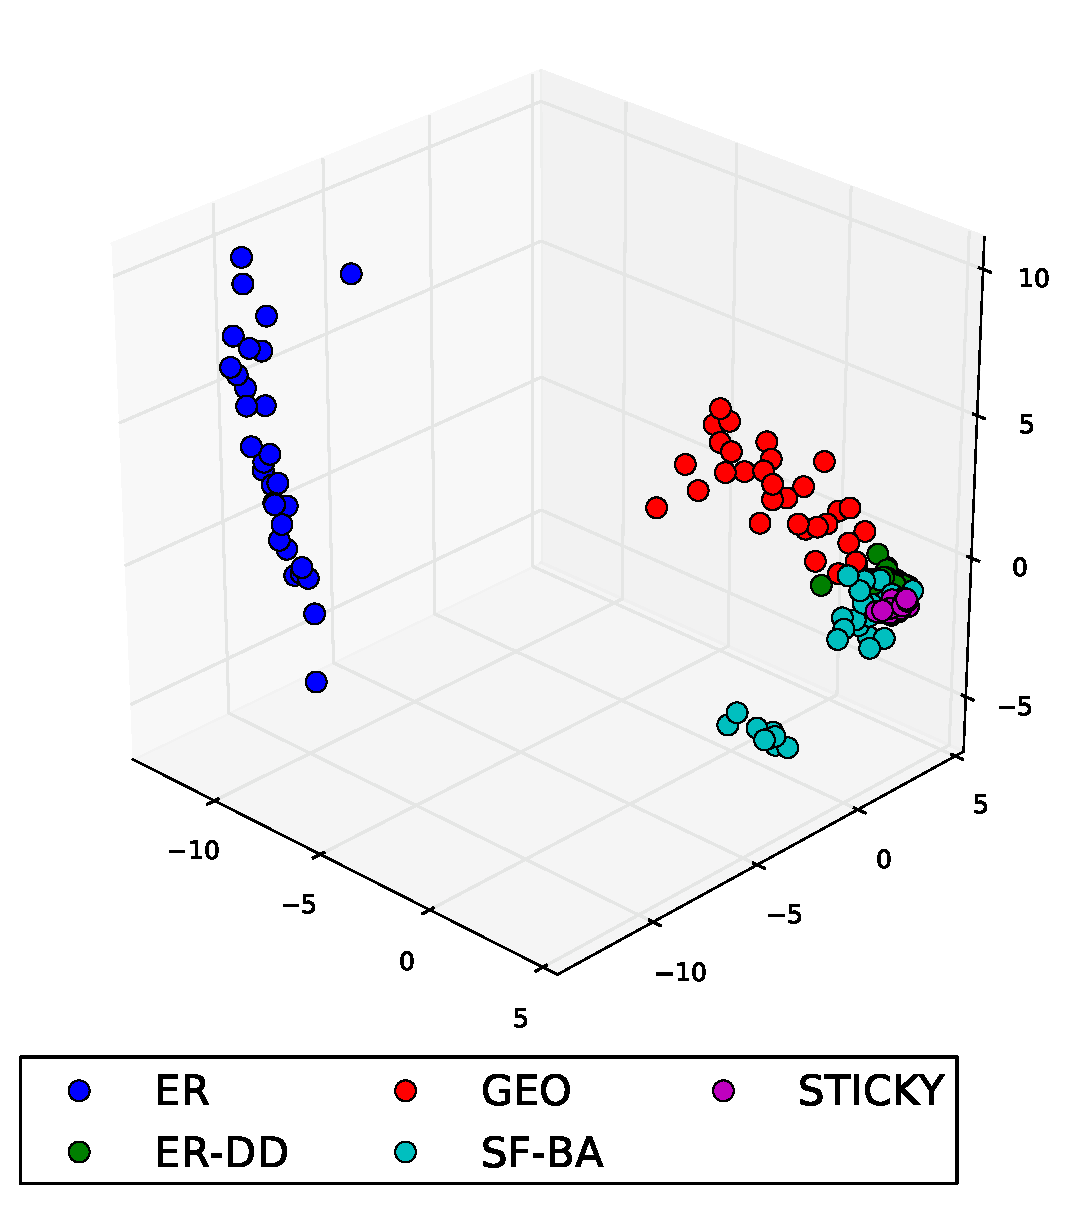
\includegraphics[scale=0.30]
    {../code/final_results/trade_2010_thresholded/eval_results/gcv_mds.pdf}
    \caption[Graphlet Cluster Vector MDS]{GCV MDS}
    \label{fig:gcv_mds}
%     \vspace{0.0ex}
  \end{minipage}%%
%   \hspace{-0.5em}
  \begin{minipage}[b]{0.50\linewidth}
    \centering
    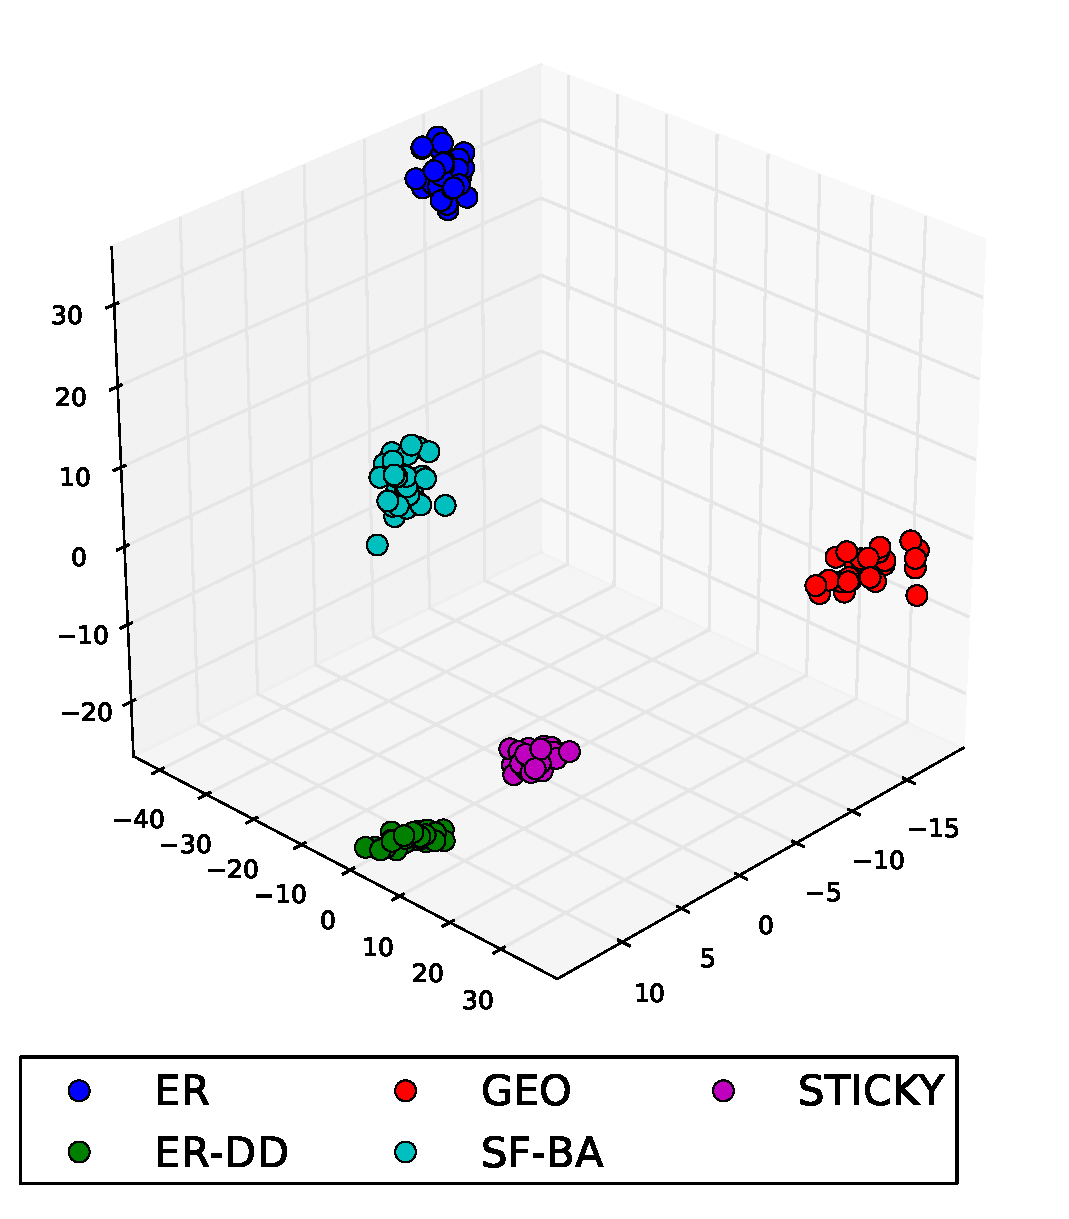
\includegraphics[scale=0.30]
    {../code/final_results/trade_2010_thresholded/eval_results/rgfd_mds.pdf}
    \caption[Clustering Coefficient MDS]{RGFD MDS}
    \label{fig:clust_coeff_mds}
%      \vspace{-1.0ex}
  \end{minipage} 
\label{fig:gcv_clust_mds} 
\end{figure}
  
  
\end{frame}

\begin{frame}
  \frametitle{Precision-Recall Curve Analysis}
  
  \begin{figure}
    \centering 
    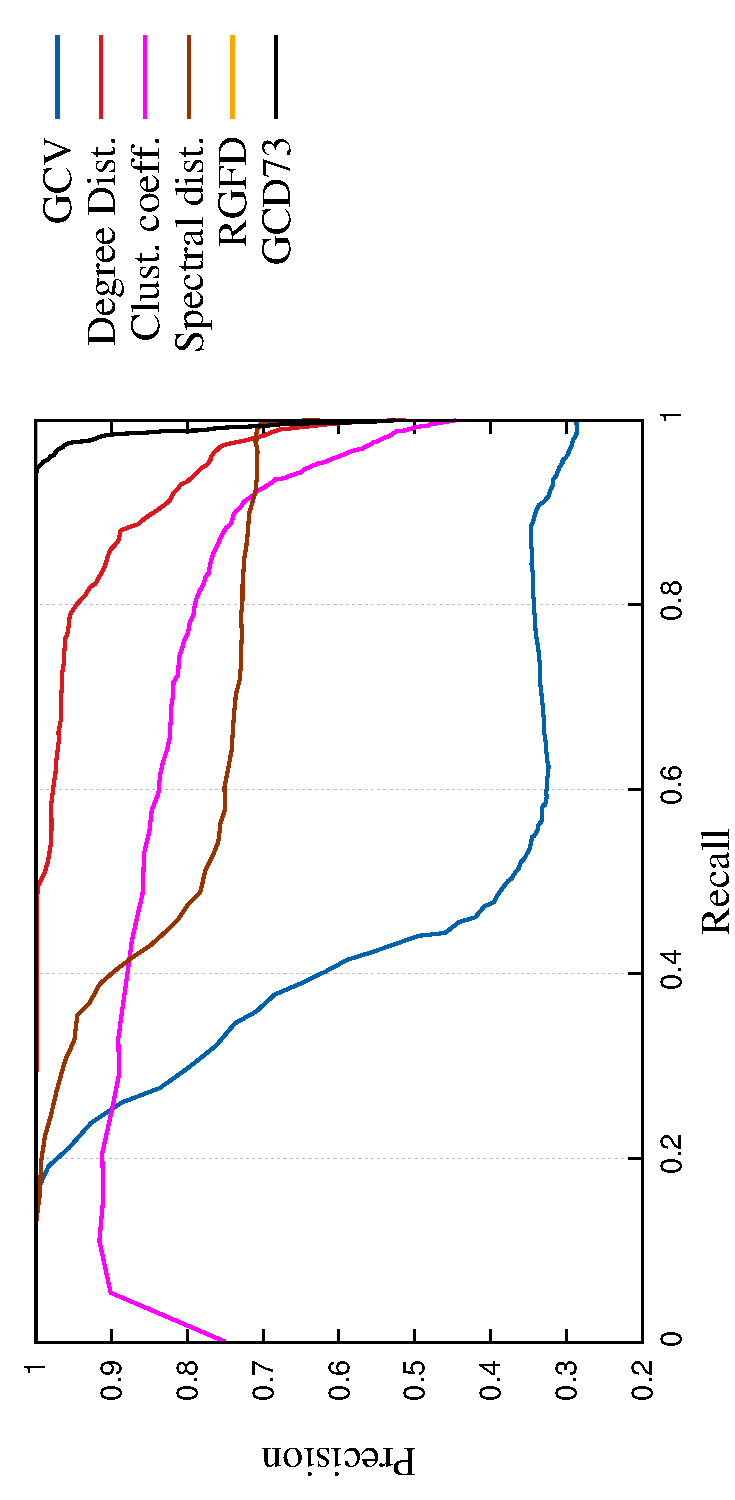
\includegraphics[scale=0.48, angle=-90]
  {../code/final_results/trade_2010_thresholded/eval_results/prec_rec_all_rnd_rew_02.pdf}
  \end{figure}

\end{frame}

\begin{frame}
  \frametitle{Robustness testing -- Noisy data}
  
  \begin{figure}
    \centering 
    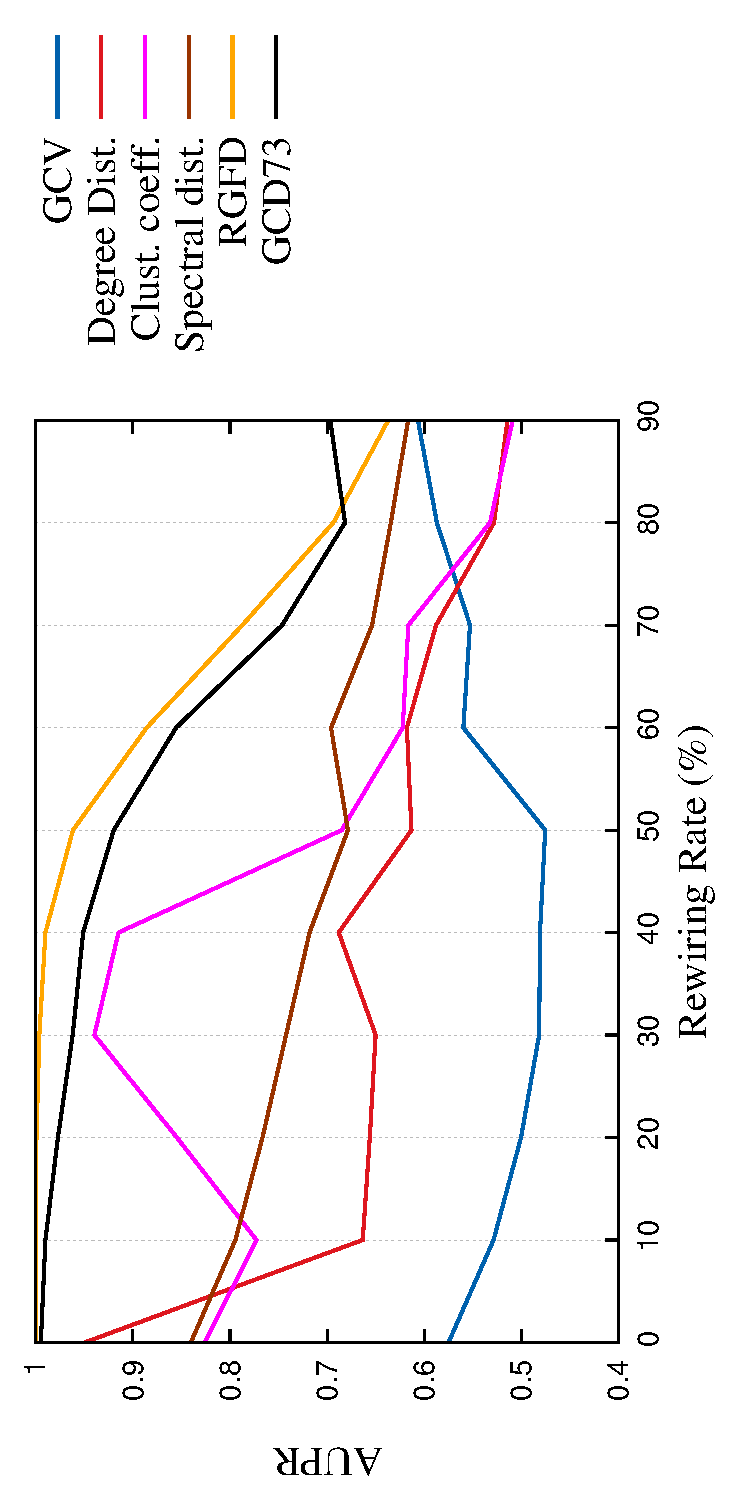
\includegraphics[scale=0.48, angle=-90]
  {../code/final_results/trade_2010_thresholded/eval_results/rew_aupr_all_sigs2.pdf}
  \end{figure}

\end{frame}

\begin{frame}
  \frametitle{Robustness testing -- Noisy and incomplete data}
  
  \begin{figure}
    \centering
    \begin{tikzpicture}
      \node (label) at (0,0) {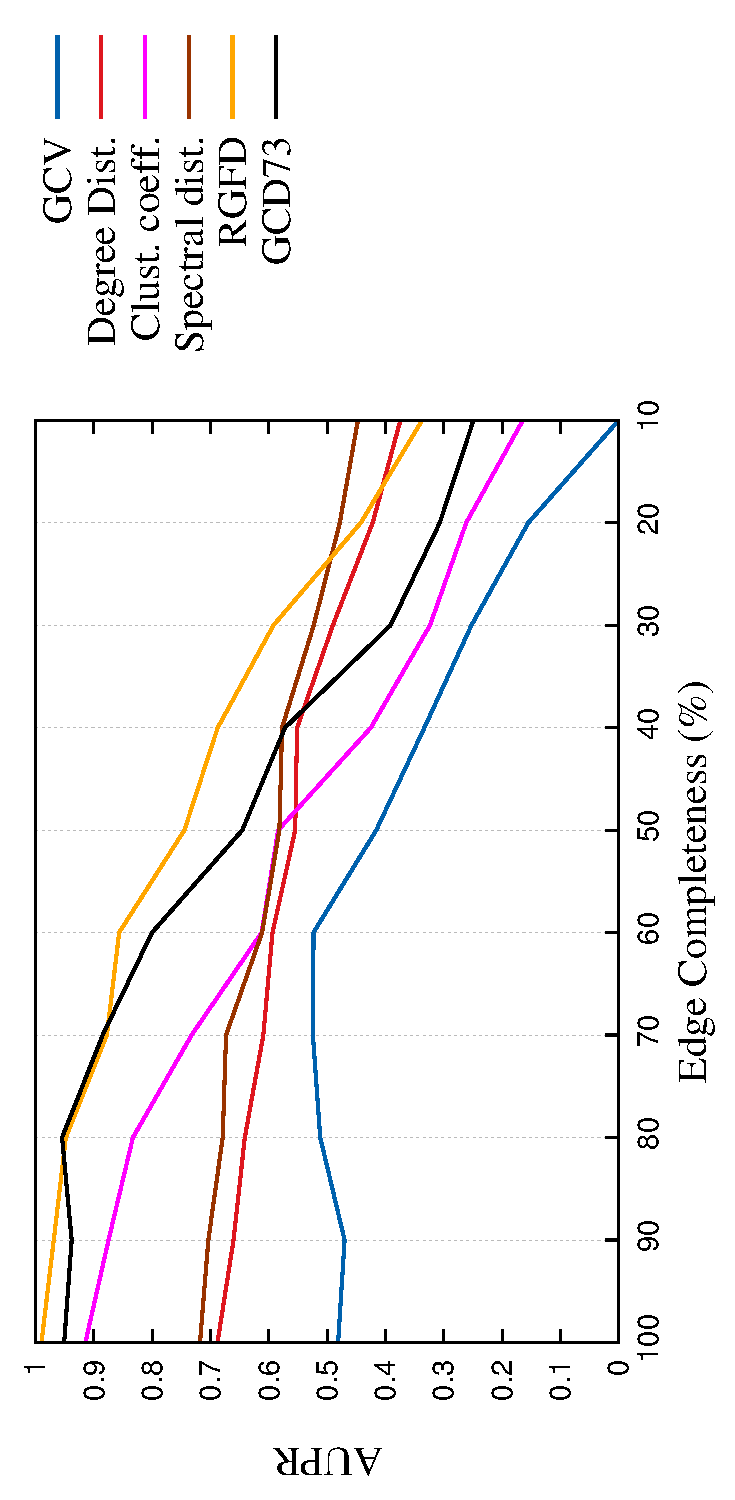
\includegraphics[scale=0.48, angle=-90]
    {../code/final_results/trade_2010_thresholded/eval_results/compl_aupr_all_sigs2.pdf}};
      \node (label) at (1,2.3) {40\% rewired};    
    \end{tikzpicture}
  \end{figure}


\end{frame}

\begin{frame}
  \frametitle{Signature approximation}
  
  \begin{figure}
    \centering    
    \begin{tikzpicture}
      \node (label) at (0,0) {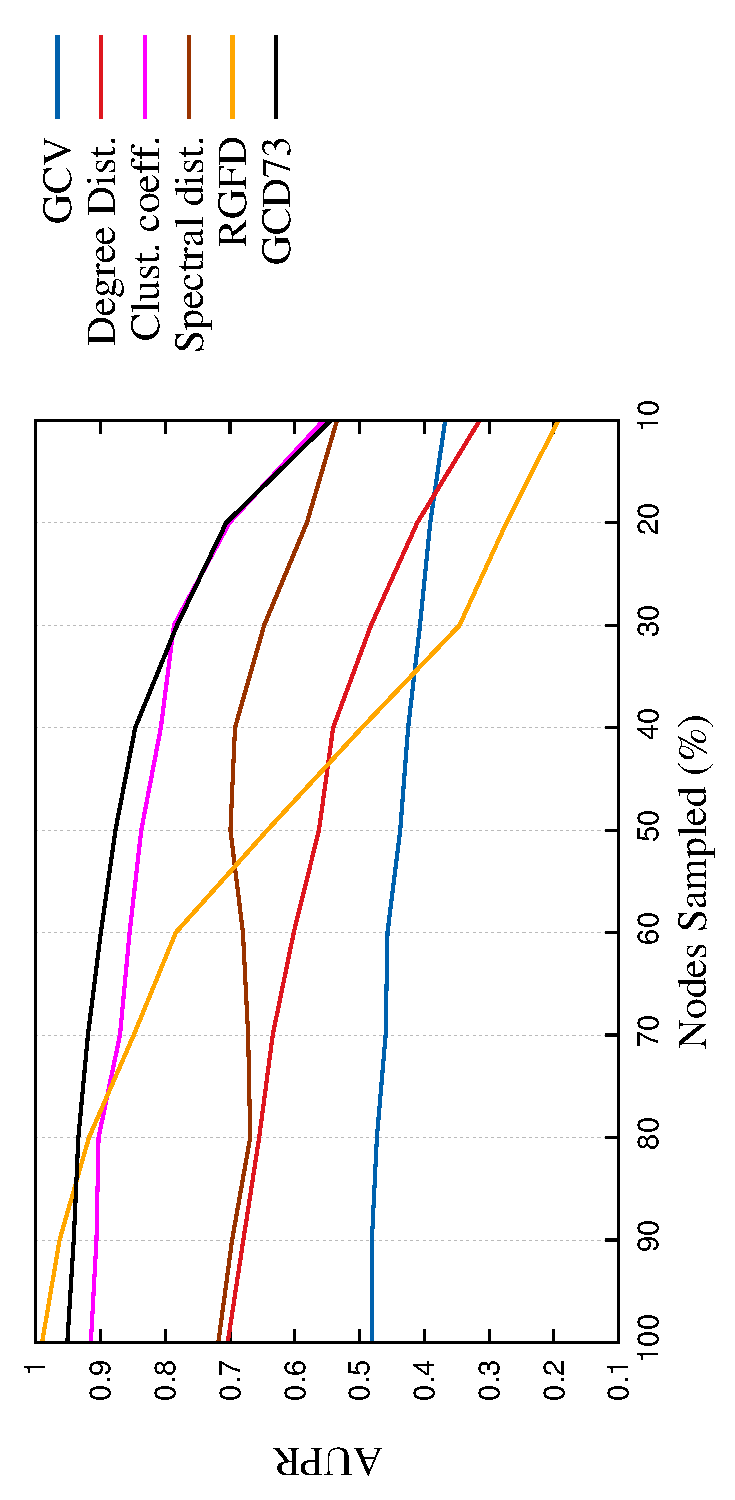
\includegraphics[scale=0.48, angle=-90]
    {../code/final_results/trade_2010_thresholded/eval_results/sampl_aupr_all_sigs2.pdf}};
      \node (label) at (1,2.3) {40\% rewired};    
    \end{tikzpicture}
  \end{figure}

  
  
\end{frame}


\begin{frame}
 \frametitle{Conclusion}
 
 \begin{itemize}
  \item GCV Implementation \vfill
  \item Applications \vfill
  
  \begin{figure}
    \hspace{-3em}
    \begin{tikzpicture}[scale=0.7,auto,swap]


    \node[inner sep=0pt] (trade) at (-5.5, 0.5) {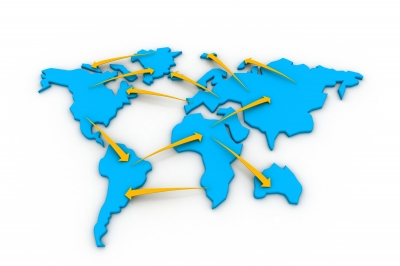
\includegraphics[width=0.33\textwidth]{images/world_trade_net.jpg}};
    \node[inner sep=0pt] (ppi) at (0, 0.0) {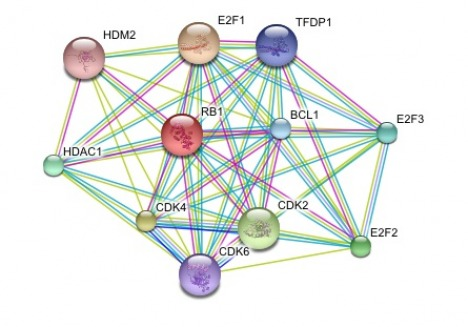
\includegraphics[width=0.33\textwidth]{images/protein_network.jpg}};
    \node[inner sep=0pt] (meta) at (5.5, 0.0) {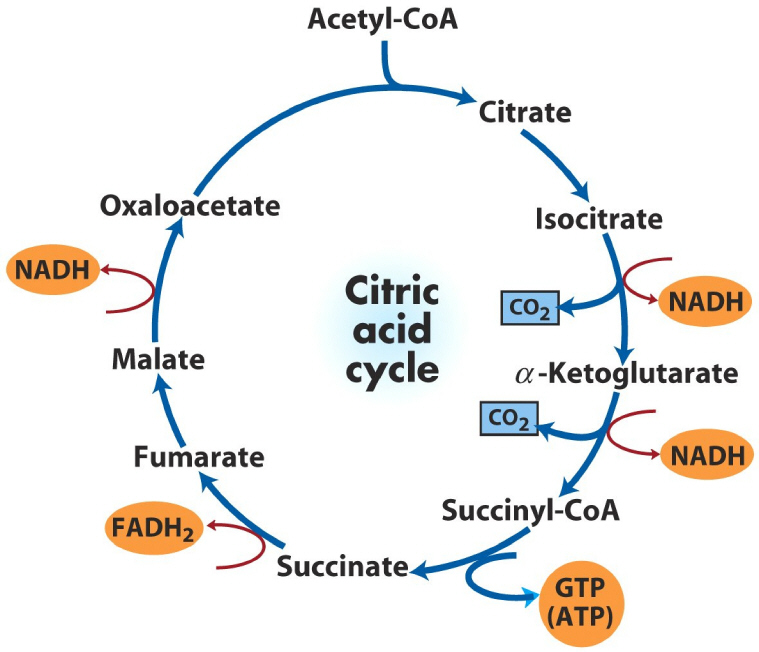
\includegraphics[scale=0.5]{images/metabolic_net.jpg}};

    \node[inner sep=0pt] (trade_label) at (-5.5,3) {\begin{tabular}{c} World Trade\\ networks \end{tabular}};
    \node[inner sep=0pt] (ppi_label) at (0,3) {\begin{tabular}{c} Protein Interaction\\ networks \end{tabular}};
    \node[inner sep=0pt] (meta_label) at (5.5,3) {\begin{tabular}{c} Metabolic\\ networks \end{tabular} };

    \end{tikzpicture}
  \end{figure}
  \item Evaluation on random graphs clustering \vfill
 \end{itemize}
 
\end{frame}

\begin{frame}
 \frametitle{Future work}
 
 \begin{itemize}
  \item Research better normalisation procedures  \vfill
  \item Redundancy analysis \vfill
  \item Supporting experiments for our current results \vfill
  \item Apply the signature to other networks \vfill
  \begin{itemize}
   \item Social networks \vfill
   \item Telecommunication networks \vfill
   \item Gene Regulatory networks \vfill
   \item Neuronal networks \vfill
  \end{itemize}

 \end{itemize}

\end{frame}

\begin{frame}
  \frametitle{Questions?}
 \vfill
 \begin{itemize}
  \item Thank you very much!
 \end{itemize}
 \vfill
 
\end{frame}

\begin{frame}
  \frametitle{GCV normalisation}
  
  \begin{itemize}
   \item normalised GCV: $$ GCV(n) = \left(F_n^1, F_n^2, ... F_n^{29}\right)$$
 where
 $$ F_n^i = \frac{S_n^i}{\sum_{i=1}^{n}S_n^i} $$
  \item all the World Trade network results presented here use the normalised GCV
  \end{itemize}

  
\end{frame}


\rowcolors{1}{}{}

\begin{frame}
  \frametitle{Limitations of the GCV signature}
  
  \begin{figure}[H]
\centering
  \begin{subfigure}[b]{0.45\textwidth}
    \begin{tikzpicture}[scale=0.8,auto,swap, every node/.style={scale=0.6}]

      \draw (1.5,0) ellipse (0.7cm and 1.7cm);
%       \node[upper left] at (current bounding box.north east) {\textbf{$S_1$}};	
      
      \node[vertex,blue] (1a) at (0,0) {$1$};
      
      % define the round nodes
      \foreach \pos/\name/\label in {
	{(1.5,0)//2a},
	{(1.5,1)//3a},
	{(1.5,-1)//4a},
	{(3,0)//5a},
	{(3,2)//6a},
	{(3,-2)//7a}}
	\node[vertex] (\label) at \pos {$\name$} ;
  
      \node[upper left,inner sep=0] (src_lab) at (-1.5,0.75) {\begin{tabular}{r} source\\ node \end{tabular}};
      \draw[->, thick]  (src_lab)  -- (1a) {}; 
	
      %neighbouring graph
	    
      \path[lo, line width=1.0]  (1a)  -- (2a);
      \path[lo, line width=1.0]  (1a)  -- (3a);
      \path[lo, line width=1.0]  (1a)  -- (4a);
      \path[hi, line width=1.0]  (2a)  -- (4a);
      \path[lo, line width=1.0]  (3a)  -- (6a);
      \path[lo, line width=1.0]  (3a)  -- (5a);
      \path[lo, line width=1.0]  (4a)  -- (7a);   
      \path[lo, line width=1.0]  (5a)  -- (7a); 
      \path[lo, line width=1.0]  (5a)  -- (6a); 
      % rest of edges, dotted

%       \path[lo, line width=1.0]  (1a)  -- (2a);
%       \path[lo, line width=1.0]  (1a)  -- (3a);
%       \path[lo, line width=1.0]  (1a)  -- (4a);
%       \path[lo, line width=1.0]  (1a)  -- (5a);
%       \path[lo, line width=1.0]  (6a)  -- (5a);
    \end{tikzpicture}
    \caption{Shell-1 neighbourhood}
    \vspace{1em}  
  \label{fig:shell1}
  \end{subfigure}
  \begin{subfigure}[b]{0.45\textwidth}
    \begin{tikzpicture}[scale=0.8,auto,swap, every node/.style={scale=0.6}]

      \draw (3,0) ellipse (0.7cm and 2.5cm);
%       \node[upper left] at (current bounding box.north east) {\textbf{$S_1$}};	
      
      \node[vertex,blue] (1a) at (0,0) {$1$};
      
      % define the round nodes
      \foreach \pos/\name/\label in {
	{(1.5,0)//2a},
	{(1.5,1)//3a},
	{(1.5,-1)//4a},
	{(3,0)//5a},
	{(3,2)//6a},
	{(3,-2)//7a}}
	\node[vertex] (\label) at \pos {$\name$} ;
  
      \node[upper left,inner sep=0] (src_lab) at (-1.5,0.75) {\begin{tabular}{r} source\\ node \end{tabular}};
      \draw[->, thick]  (src_lab)  -- (1a) {}; 
	
      %neighbouring graph
	    
      \path[lo, line width=1.0]  (1a)  -- (2a);
      \path[lo, line width=1.0]  (1a)  -- (3a);
      \path[lo, line width=1.0]  (1a)  -- (4a);
      \path[lo, line width=1.0]  (2a)  -- (4a);
      \path[lo, line width=1.0]  (3a)  -- (6a);
      \path[lo, line width=1.0]  (3a)  -- (5a);
      \path[lo, line width=1.0]  (4a)  -- (7a);   
      \path[hi, line width=1.0]  (5a)  -- (7a); 
      \path[hi, line width=1.0]  (5a)  -- (6a); 
      % rest of edges, dotted

%       \path[lo, line width=1.0]  (1a)  -- (2a);
%       \path[lo, line width=1.0]  (1a)  -- (3a);
%       \path[lo, line width=1.0]  (1a)  -- (4a);
%       \path[lo, line width=1.0]  (1a)  -- (5a);
%       \path[lo, line width=1.0]  (6a)  -- (5a);
    \end{tikzpicture}
    \caption{Shell-2 neighbourhood} 
    \vspace{1em}  
    \label{fig:shell2}
  \end{subfigure}
\label{fig:shell_core}
\end{figure}
  
  \begin{itemize}
   \item the GCV cannot capture information in nodes that are at a distance of 2 or larger away from the source node
   \item some of the GCV frequencies might be redundant
   \item computation of the GCV is slow on very dense networks such as the full WTN
  \end{itemize}

\end{frame}

\begin{frame}
 \frametitle{Signatures evaluated -- definitions}
 
 \begin{itemize}
  \item Spectral distribution: eigenvalues $(\lambda_1, \lambda_2, \dots, \lambda_n)$ of the Laplacian matrix $L = D - A$ where:
  \begin{itemize}
   \item $D$: diagonal degree matrix of $G$ 
   \item $A$: adjacency matrix
  \end{itemize}
  \item Graphlet Frequency vector: $GFV(G) = \left(F_0(G), F_1(G), ... F_{29}(G)\right) $ where:
  \begin{itemize}
    \item $ F_i(G) = -\log\left(\frac{G_i}{\sum_{i=1}^{n}G_i}\right) $
    \item $G_i$ is the total number of graphlets of type $i$ in $G$
  \end{itemize}
  \item Graphlet Distribution Vector of node $x$: a vector $ (F_1, F_2, \dots, F_{72}) $, where:
  \begin{itemize}
    \item $f_i$ measures the number of graphlets that touch node $x$ at automorphism orbit $i$.
  \end{itemize}
 \end{itemize}

\end{frame}



 
\newcommand{\ccaIndicatorsPPI}{
% \begin{table}
%   \small
  \begin{tabular}{>{\large}r}
  \cellcolor{black}\textcolor{ccacol0}{Ribosome translation}\\
  \cellcolor{black}\textcolor{ccacol4}{RNA processing}\\
  \cellcolor{black}\textcolor{ccacol5}{Protein degradation}\\
  \cellcolor{black}\textcolor{ccacol5}{Cell cycle}\\
  \cellcolor{black}\textcolor{ccacol5}{Nuclear transport}\\
  \cellcolor{black}\textcolor{ccacol5}{ER Golgi traffic}\\
  \cellcolor{black}\textcolor{ccacol5}{Protein folding}\\
  \cellcolor{black}\textcolor{ccacol5}{Chromatin segmentation}\\
  \cellcolor{black}\textcolor{ccacol5}{Signalling stress response}\\
  \cellcolor{black}\textcolor{ccacol5}{Cell polarity morphogenesis}\\
  \cellcolor{black}\textcolor{ccacol5}{Chromatin transcription}\\
  \cellcolor{black}\textcolor{ccacol5}{DNA replication}\\
  \cellcolor{black}\textcolor{ccacol5}{Metabolism -- mitochondria}\\
  \cellcolor{black}\textcolor{ccacol6}{Golgi endosome sorting}
  \end{tabular}
% \end{table}
}

\begin{frame}

\frametitle{Protein interaction network CCA}

\begin{figure}[H]
  \centering
    \begin{tikzpicture}[scale=\ccafigscaleppi,show background rectangle, 
  background rectangle/.style={fill=black},
  color=white,help lines/.style={color=lightgray,line width=0.2pt},post/.style={->,shorten >=1pt,>=stealth',thick}]

    \node[upper left,inner sep=0,scale=\ccafigscaleppi * 1.3] (indicators) at (-2.5,0) {\ccaIndicatorsPPI};	
    \shade[top color=green,bottom color=yellow] (4,0) rectangle (4.5,5);
    \shade[top color=yellow,bottom color=red] (4,-5) rectangle (4.5,0);
    \node[upper left,inner sep=0] (dummy) at (14.0,4) {}; % for extending the black bounding box
%     \node[upper left,inner sep=0] (dummy2) at (-8.0,4) {}; % for extending the black bounding box
    \node[upper left,inner sep=0,scale=\ccafigscaleppi * 1.3] (corr_text) at (4.25,-6.0) {Correlation};
    \node[upper left,inner sep=0,red] (corr_text) at (4.25,-5.5) {-1};
    \node[upper left,inner sep=0, green] (corr_text) at (4.25,5.5) {1};
    \node[upper left,inner sep=0] (corr_text) at (4.75,0) {0};
    
    \node[upper left,inner sep=0,scale=\ccafigscaleppi] (g2) at (7.5,5) {\gtwocca{ccacol1}};
    \node[upper left,inner sep=0,scale=\ccafigscaleppi] (g8) at (10.5,3.5) {\geightcca{ccacol1}};
    \node[upper left,inner sep=0,scale=\ccafigscaleppi] (g29) at (7.5,2) {\gtwentyninecca{ccacol1}};
    \node[upper left,inner sep=0,scale=\ccafigscaleppi] (g13) at (10.5,-2.5) {\gthirteencca{ccacol3}};
    \node[upper left,inner sep=0,scale=\ccafigscaleppi] (g10) at (7.5,-4) {\gtencca{ccacol3}};
    \node[upper left,inner sep=0,scale=\ccafigscaleppi] (g9) at (11.5,-5.5) {\gninecca{ccacol3}};
    
    \draw[line,color=white] (6,0) -- (13.00,0);
    \node[upper left,inner sep=0,scale=\ccafigscaleppi * 1.3] (strong_corr) at (10,0.5) {Highest correlations};    
    \node[upper left,inner sep=0,scale=\ccafigscaleppi * 1.3] (strong_corr) at (10,-0.5) {Lowest correlations};    
    
%     \draw[line,color=ccacol0] (0.85,4.10) -| (1.15,4.58) -- (4.00,4.58);
%     \draw[line,color=ccacol0] (0.85,3) -| (1.15,4.58) -- (4.00,4.58);

    \draw[line,color=ccacol0] (0.85,4.10) -| (1.89,4.58) -- (4.00,4.58);
    \draw[line,color=ccacol4] (0.85,3.47) -| (3.73,0.43) -- (4.00,0.43);
    \draw[line,color=ccacol5] (0.85,2.84) -| (3.16,-0.07) -- (4.00,-0.07);
    \draw[line,color=ccacol5] (0.85,2.21) -| (2.85,-0.09) -- (4.00,-0.09);
    \draw[line,color=ccacol5] (0.85,1.58) -| (2.67,-0.38) -- (4.00,-0.38);
    \draw[line,color=ccacol5] (0.85,0.95) -| (2.40,-0.51) -- (4.00,-0.51);
    \draw[line,color=ccacol5] (0.85,0.32) -| (2.07,-0.51) -- (4.00,-0.51);
    \draw[line,color=ccacol5] (0.85,-0.31) -| (1.79,-0.60) -- (4.00,-0.60);
    \draw[line,color=ccacol5] (0.85,-0.94) -| (1.79,-0.64) -- (4.00,-0.64);
    \draw[line,color=ccacol5] (0.85,-1.57) -| (2.08,-0.72) -- (4.00,-0.72);
    \draw[line,color=ccacol5] (0.85,-2.20) -| (2.41,-0.73) -- (4.00,-0.73);
    \draw[line,color=ccacol5] (0.85,-2.83) -| (2.67,-0.85) -- (4.00,-0.85);
    \draw[line,color=ccacol5] (0.85,-3.46) -| (3.40,-0.86) -- (4.00,-0.86);
    \draw[line,color=ccacol6] (0.85,-4.09) -| (3.66,-1.00) -- (4.00,-1.00);


    
    
    \draw[line,color=ccacol1] (g2) -| (5.5,4.5) -- (4.5,4.5);
    \draw[line,color=ccacol1] (g8) -| (5.9,4.4) -- (4.5,4.4);
    \draw[line,color=ccacol1] (g29) -| (5.7,4.3) -- (4.5,4.3);

    \draw[line,color=ccacol3] (g13) -| (5.5,2.3) -- (4.5,2.3);
    \draw[line,color=ccacol3] (g10) -| (5.3,2.2) -- (4.5,2.2);
    \draw[line,color=ccacol3] (g9) -| (5.1,2.1) -- (4.5,2.1);
    
    \end{tikzpicture}
    \label{fig:ppi_cca_black}	
\end{figure}

 
\end{frame}

\begin{frame}
 \frametitle{Pearson's and Spearman's correlation coefficients}
 
 \begin{itemize}
  \item Pearson's correlation coefficient between $X$ and $Y$:\vfill
    \begin{itemize}
     \item $ \rho_{X,Y} = \frac{\sigma_{XY}}{\sigma_X\sigma_Y} = \frac{E[X-\mu_X]E[Y-\mu_Y]}{\sigma_X\sigma_Y}$ \vfill
    \end{itemize}
  \item Spearman's correlation coefficient between $X$ and $Y$:\vfill 
  \begin{itemize}
   \item each data point $X_i$ and $Y_i$ is converted to their ranks $R^X_i$ and $R^Y_i$ \vfill
   \item the Pearson's correlation coefficient between $R_X$ and $R_Y$ is computed \vfill
  \end{itemize}

 \end{itemize}

 
\end{frame}



\end{document}